%%%%%%%%%%%%%%%%%%%%%%%%%%%%%%%%%%%% PREAMBOLO - INIZIO %%%%%%%%%%%%%%%%%%%%%%%%%%%%%%%%%%%%%%%%%%%%%%%%%%%
\documentclass[a4paper,12pt]{report}

%%%%%%%%%%% PACCHETTI %%%%%%%%%%
\usepackage[utf8]{inputenc}
\usepackage[T1]{fontenc}
\usepackage[italian]{babel}
\usepackage{graphicx}	% per le immagini
\usepackage{fancyhdr}	% per le impostazioni della pagina
\usepackage{amsmath} %<--pacchetto American Mathematician Society
\usepackage{amssymb} %<--pacchetto piu' ampio per simboli matematici
\usepackage[pdftex,bookmarks=true]{hyperref} % per gli hyperlinks
\usepackage{boxedminipage} % for boxed paragraphs

% PACCHETTO MOLTO CONSIGLIATO! Serve ad impostare i margini in modo professionale!
%\usepackage{layaureo}	% Il layout della tesi (richiede il pacchetto aggiuntivo LayAureo)

%%%%%%%%%%%%%%%%%%%%%%%%%%%%%%%%

% Carattere Bitstream Character
\renewcommand{\familydefault}{bch}

% Assicura che le eventuali pagine bianche non abbiano intestazioni e pie' di pagina
\clearpage{\pagestyle{empty}\cleardoublepage}

% numerazione delle pagine "araba"
\pagenumbering{arabic}

%%%%%%%%%%%%%%%%%%%%%%%%%%%%%%%%% PREAMBOLO - FINE %%%%%%%%%%%%%%%%%%%%%%%%%%%%%%%%%%%%%%%%%%%%%%%%%%%%



%%%%%%%%%%%%%%%%%%%%%%%%%%%%%%%%% DOCUMENTO - INIZIO %%%%%%%%%%%%%%%%%%%%%%%%%%%%%%%%%%%%%%%%%%%%%%%%%%
\begin{document}
	
	% New commands
	\newcommand{\visualnetkit}{\emph{VisualNetkit}}
	\newcommand{\emulazione}{\emph{emulazione}}
	\newcommand{\linux}{\emph{Linux}}
	\newcommand{\windows}{\emph{Windows}}
	\newcommand{\testbed}{\emph{testbed}}
	\newcommand{\simulazione}{\emph{simulazione}}
	\newcommand{\virtualmachine}{\emph{Virtual Machine}}
	\newcommand{\netkit}{\emph{NetKit}}
	\newcommand{\xml}{\emph{XML}}
	\newcommand{\plugin}{\emph{Plug-In}}
	\newcommand{\stakeholders}{\emph{stakeholders}}
	\newcommand{\bu}{\emph{Bottom-Up}}
	\newcommand{\qt}{\emph{Qt}}
	\newcommand{\cpp}{\emph{C++}}


	% alcune parole: sillabazione
	\hyphenation{up-load} 
	
	% Ridefinisco localmente lo stile plain (ovvero lo stile che usa la prima
	% pagina di ogni capitolo), per nascondere il numero della
	% pagina anche all'inizio di Prefazione e Indice.
	\fancypagestyle{plain}{%
		\fancyhf{}
		\renewcommand{\headrulewidth}{0pt}
	}
	
	\addtolength{\skip\footins}{2em}	%Spaziatura testo - footnota
		
	\baselineskip=16pt	%L'interlinea 1.5 circa
	\pagestyle{empty}

	%%%%%%%%%%% FREONTESPIZIO DEDICA ED INDICE %%%%%
	\begin{figure}[!h]
	\centering
	\includegraphics[width=3cm]{images/logo_uni.png}
\end{figure}
\begin{center}
	\begin{Large}Università degli studi di ``Roma Tre''\end{Large}\\
	\vspace{0.5cm}
	\begin{Large}\textbf{Facoltà di Ingegneria}\end{Large}\\
	\vspace{0.5cm}
	\begin{Large}Corso di Laurea Magistrale in Ingegneria Informatica\end{Large}\\
	\vspace{2cm}
	\begin{huge}Progettazione e Realizzazione di un Ambiente per la Configurazione Avanzata di Reti Virtuali\end{huge}\\
	\vspace{1.5cm}
	\begin{large}Tesi finale\end{large}\\
	\vspace{2cm}	
	\begin{tabular}{cc}
		\begin{minipage}{6.5cm}
			\centering
			Relatore
		\end{minipage}
		&
		\begin{minipage}{6.5cm}
			\centering
			Laureando\\
		\end{minipage}
		\\
		\begin{minipage}{6.5cm}
			\centering
			\vspace{0.4cm}
			\textbf{\textit{Prof. Maurizio Pizzonia}}
		\end{minipage}
		&
		\begin{minipage}{6.5cm}
			\centering
			\textbf{\textit{Alessio Di Fazio}}
		\end{minipage}
		\\
		\begin{minipage}{6.5cm}
			\centering
			\vspace{1cm}
			Correlatore
		\end{minipage}
		\\
		\begin{minipage}{6.5cm}
			\centering
			\vspace{0.4cm}
			\textbf{\textit{Dott. Massimo Rimondini}}
		\end{minipage}
	\end{tabular}

	\vspace{1.5cm}%
	\begin{minipage}{8cm}
		\centering
		Anno accademico 2007/2008
	\end{minipage}
\end{center}



	% inizio tesi senza intestazione di pagina e pie' di pagina
	
	\null\vspace{\stretch{1}}
\begin{flushright}
	\begin{Small}
	\textit{Alla mia famiglia che mi ha dato la possibilità di laurearmi.} \\
	\textit{A me per la mia tenacia e forza di volontà.} \\
	\textit{A tutte quelle persone che non hanno mai creduto in me! :)} \\
	\end{Small}
\end{flushright}
\vspace{\stretch{1}}\null

	\tableofcontents	% l'indice
	% Inserisce la voce di questo capitolo nell'indice
	\addcontentsline{toc}{chapter}{Indice}
	
	%%%%%%%%%%%%%%%%%%%%%%%%%%%%%%%%%%%%%%%%%
	
	%%%%%%%%%%%%%%%%%%%%%%%%%%%%%%%%%%%%%%%%%
	% PREFAZIONE
	%%%%%%%%%%%%%%%%%%%%%%%%%%%%%%%%%%%%%%%%%	
	\chapter*{Introduzione}
% Inserisce la voce di questo capitolo nell'indice
\addcontentsline{toc}{chapter}{Introduzione}
TODO
		
	% Le righe seguenti impostano la struttura che avra' tutto il resto della tesi
	
	\fancypagestyle{plain}{%	% ripristino il numPag nell'ambiente plain
		\fancyhf{}
		\cfoot{\thepage}
		\renewcommand{\headrulewidth}{0pt}
	}
	% Imposto intestazione e pie' di pagina della altre pagine
	\pagestyle{fancy}	
	\rhead{\footnotesize\bfseries\leftmark}
	\lhead{\footnotesize\chaptername \ \thechapter}
	
	%%%%%%%%%%%%%%%%%%%%%%%%%%%%%%%%%%%%%%%%%
	% CAPITOLO 1
	%%%%%%%%%%%%%%%%%%%%%%%%%%%%%%%%%%%%%%%%%
	\chapter{Stato dell'arte}\label{capitolo:arte}
\markboth{Stato dell'arte}{}

In questo capitolo di apertura vogliamo fornire una breve descrizione dei sistemi di \emulazione{} di reti di computers esistenti mettendoli a confrondo per capire le loro potenzialità; in parlicolar modo verrà descritto come questi si comportano davanti ad un utente che vuole creare configurazioni per reti complesse.

Nella seconda parte verranno discusse le qualità della prima release\footnote{Release, letteralmente ``rilascio'', in ambito informatico indica una particolare versione di un software resa disponibile ai suoi utenti, univocamente identificata da altre particolari versioni rese disponibili in precedenza da un particolare numero di versione.} di \visualnetkit{} e, come si vedrà nei successivi capitoli, verranno enfatizzati i punti deboli di questa prima versione che verrà messa a paragone con le pontenzialità offerte dal nuovo e più flessibile ambiente offerto dalla nuova release.

\section{Panoramica sui sistemi di \emulazione{}}
Prima di concentrare i nostri sforzi sul capire cosa rappresenta un ``ambiente di \emulazione{}'' focalizziamo l'attenziene sul significato stesso della parola \emulazione{}. Un software di \emulazione{} o più comunemente chiamato ``emulatore'' è un programma che permette l'esecuzione di software scritto per un ambiente (hardware o software) diverso da quello sul quale l'emulatore stesso viene eseguito.

Un programma scritto e compilato per una determinata piattaforma software (ad esempio \windows) non viene eseguito su un computer con sistema operativo differente come \linux{}. In questi casi si crea sulla macchina ospitante ``Host'' un emulatore che riproduce virtualmente l'ambiente che è stato usato per creare quel programma (nel nostro esempio un ambiente \windows{}). Il sistema virtuale che gira all'interno di quello emulato viene chamato sistema ``Guest''.

I sistemi di \emulazione{} di reti nascono con l'intento di riprodurre il funzionamento delle reti reali e di tutti i servizi che esse offrono agli utenti; configurazioni particolari, protocolli, ecc\ldots

Una rete di calcolatori può essere definita come un sistema informatico costituito da due o più calcolatori che, collegati tra loro tramite un mezzo trasmissivo, possono scambiarsi informazioni di vario genere. Naturalmente nella realtà le cose sono molto più complesse che una semplice definizione. Proprio per questo motivo un sistema di \emulazione{} deve offrire la possibilità di gestire qualsiasi configurazione e comportamento che i calcolatori presenti in rete possono assumere, permettendo così una rappresentazione eterogenea di macchine che offrono diversi servizi e svolgono diverse attività.

I sistemi attualmente esistenti permettono la creazione di reti composte da centinaia di computers generando, di conseguenza, un proporzionale aumento di macchine interfaccie di rete e protocolli coinvolti.

\subsubsection{Ma perché emulare reti di calcolatori?}
Lo scopo principale di un sistema di \emulazione{} di reti di calcolatori è quello di riprodurre e sperimentare il funzionamento dei nodi\footnote{Per ``nodo'' in una rete di calcolatori si intendono computers provvisti di memoria.} e dei connettori\footnote{Per ``connettore'' si intendono dispositivi come ad esempio hub, bridge, ecc\ldots}, al fine di testare nuovi protocolli e verificare il corretto funzionamento della rete. Tutto questo viene affrontato in maniera ``virtuale'' senza dover acquistare dispositivi spesso molto costosi.

Si pensi ad esempio all'ambito didattico; lo studente (o il ricercatore, o l'individuo che vuole studiare e sperimentare reti di calcolatori) dovrebbe dapprima studiare la soluzione ``su carta'', acquistare le dovute apparecchiature di rete (che come noto hanno un impatto economico non trascurabile), assemblare la rete, configurare adeguatamente ogni singolo nodo e connettore della rete e solamente alla fine passare alla fase di test sulla rete assemblata. E cosa succede se lo studente volesse modificare una parte della rete? Da questo si evince immediatamente che questo scenario nella maggior parte dei casi non è praticabile e come l'uso dei sistemi di \emulazione{} semplifichi notevolmente tali attività rendendo possibile l'intera progettazione su di un singolo calcolatore che ospita un sistema di \emulazione{}.


\subsection{Classificazione dei sistemi di \emulazione{}}
Allo stato attuale esistono molteplici tipologie di soluzioni offerte nel campo dell'\emulazione{} di sistemi. In questi ulmiti anni il bisogno di prototipi ed ambienti per la realizzazione di esperimenti nel campo delle reti di calcolatori ha catturato grande attenzione nel mondo della ricerca e dello sviluppo, dirottando notevoli sforzi in tal senso portando alla distinzione di tre principali classi di metodologie e strumenti: reti \testbed{}, \simulazione{}, \emulazione{} di reti e \virtualmachine.

Le reti \testbed{} sono ambienti costruiti su un hardware reale, come routers o hosts, interconnessi e propriamente configurati atti a realizzare la tipologia di rete desiderata. Sebbene questa soluzione è in grado di offrire un elevato grado di realismo, gli ambienti \testbed{} tendono ad essere difficilmente realizzabili per via dell'elevata difficoltà di realizzazione, mantenimento e soprattutto per costi talvolta proibitivi e raramente accessibili.

I simulatori offrono ambienti per la realizzazione di reti concettuali. Questi sono tipicamente stumenti altamente configurabili ed estensibili progettati per testare e valutare le dinamiche di rete in un ambiente disaccoppiato da ogni sorta di traffico o sistema esterno. 

Gli emulatori di reti (di cui ci occuperemo meglio più avanti) possono essere considerati un innesto di reti \testbed{} e simulatori di reti essendo in grado di riunire le caratteristiche proprie del traffico e dei sistemi coinvolti nelle reti reali. La maggior parte di essi, infatti, è costituito da un \emph{motore di emulazione} e di un interfaccia che permetta di interagire con lo stesso. Il motore dell'emulatore assolve il compito di mantenere in piedi il sistema emulato agendo a basso livello, spesso con primitive di sistema. Esso è in grado di riprodurre virtualmente tutte le componenti hardware e software, e quindi, di predisporre un ambiente standard ``gradito'' al sistema che si andrà ad emulare.

Le \virtualmachine{}, infine, si possono considerare un ``PC nel PC''. Ossia, mediante una \virtualmachine{} è possibile installare un secondo sistema operativo in una macchina virtuale e farci girare software in un ambiente considerato più ``protetto'' che non la macchina host vera e propria. Come si può immaginare, al di là della lentezza (comunque relativa e proporzionale alla potenza della macchina host), non vi è alcun limite. Questi sistemi a volte emulano anche parti di hardware, e altre volte si limitano a replicare l'hardware della macchina host. Una \virtualmachine{} solitamente è posizionata all'interno di un sistema di \emulazione{}. Quest'ultimo aspetto verrà ripreso più volte durante il corso del lavoro proposto.


\subsection{Ambienti di \emulazione{} a confronto}
Negli ultimi anni si sono affermati diversi strumenti ed ambienti di emulazione che possono essere caratterizzati sulla base delle tecniche di emulazione adottate, dei tipi di dispositivi da essi emulati o di licenza con cui sono distribuiti oltre che per le diverse funzionalità offerte.

Di seguito andremo a descrivere brevemente alcuni dei più rappresentativi in materia di emulazione di reti.

\paragraph{Imunes}\cite{OSSINI} è un software di emulazione che si avvale di una estensione del kernel \textit{FreeBSD} capace di eseguire più istanze indipendenti dello stack di rete su un unico kernel del sistema operativo. Un editor grafico della topologia di rete consente di preparare rapidamente esperimenti costituiti da apparati di rete quali hub, switch, router e host.
\begin{figure}[!ht]
	\centering
	\includegraphics[width=9cm]{images/imunes_gui_normal.png}
	\caption{GUI per il software di emulazione IMUNES.}
	\label{figura:imunes_gui}
\end{figure}

\paragraph{Marionnet}\cite{MVNL08} è anch'esso un ambiente di emulazione di reti virtuali. Permette all'utente di definire, configurare ed istanziare reti di computer anche complesse senza alcun bisogno di apparati fisici. Scritto in \textit{OCaml} ed appogginadosi su \emph{User Mode Linux}\footnote{\emph{User Mode Linux} (UML) da la possibilità di avviare varie \virtualmachine{} con sistema \linux{} (sistema ``Guest'') per eseguire applicazioni come quello che accade con un normale sistema \linux{} (sistema ``Host''). Ogni sistema guest è una normale processo avviato in \emph{user space}.} e \textit{VDE}\footnote{VDE è un  rete virtuale compatibile con ethernet che può essere configurata su una rete di computer fisici su Internet. VDE fa parte del progetto \textit{VirtualSquare}.}, offre una interfaccia grafica molto intuitiva.
\begin{figure}[!ht]
	\centering
	\includegraphics[width=9cm]{images/marionnet_gui.png}
	\caption{Finestra principale di Marionnet mostra una rete composta da tre computer, uno switch un hub ed un gateway.}
	\label{figura:marionnet_gui}
\end{figure}

\netkit{}\cite{NETKIT}  e \emph{VNUML}\cite{VNUMLT} sono entrambi emulatori di medie dimensioni che utilizzano un kernel \emph{User Mode Linux} e permettono di avere importanti esperienze in ambito di reti emulate anche complesse.

\paragraph{Netkit}In \netkit{} una rete viene modellata come la connessione di macchine virtuali. Per la creazione di un lab è necessario creare un file di configurazione per il lab stesso, in cui si descrive la topologia della rete, e alcuni file e directory per ogni virtual machine che si vuole connettere alla rete. In figura \ref{figura:netkit_lab} viene riportato un esempio di struttura di un \netkit{} laboratory.

\begin{figure}[!ht]
	\centering
	\includegraphics[width=10cm]{images/netkit_lab.png}
	\caption{Schema di rete di un semplice lab in \netkit{} con relativa configurazione.}
	\label{figura:netkit_lab}
\end{figure}

L'interazione tra l'utente finale e le macchine virtuali è possibile per mezzo di una interfaccia a riga di comando tramite terminali emulati (\linux{} shell) un po' come se si stesse davanti an usa sessione \emph{SSH}\footnote{SSH (Secure SHell, shell sicura) è un protocollo che permette di stabilire una sessione remota cifrata ad interfaccia a linea di comando con un altro host.}.


\paragraph{Vnuml}\cite{VNUMLT} (Virtual Network User Mode Linux) è un ambiente di emulazione di reti che raccoglie una serie di script utilizzati per la descrizione di \testbed{} in \xml{}, per il test di applicazioni di rete e servizi.

VNUML consiste in un linguaggio basato su \xml{}, con una specifica sintassi, e di un interprete che può essere utilizzato per descrivere ed eseguire una rete emulata di macchine virtuali UML.
Dalla descrizione in \xml{} degli scenari, VNUML istanzia le macchine virtuali UML e le configura nascondendo all'utente i dettagli avanzati e la configurazione virtuale delle macchine. Questo ambiente risulta molto utile per testare reti anche complesse. Comunque, i progettisti devono descrivere il completo scenario di rete utilizzando il linguaggio \xml{} che, a volte, richiede dettagli molto specifici.

Ad affiancare questo ambiente allo scopo di introdurre una rappresentazione grafica intuitiva è stato realizzato \emph{VNUMLGUI}\cite{VNUMLGUI}. \emph{VNUMLGUI} è un'interfaccia grafica per VNUML.
Esso è soprattutto un editor di topologia con capacità grafiche. Permette di creare qualsiasi topologia di rete virtuale in VNUML senza dover editare manualmente il file \xml{} ma con la sola immissione di router e interruttori.
Così come VNUML nasconde la curva di apprendimento di UML, \emph{VNUMLGUI} nasconde la curva di apprendimento di VNUML e \xml{}.

Di seguito sono riportati a titolo di esempio uno schema di rete e la sua corrispettiva implementazione in VNUML ed una raffigurazione dell'interfaccia grafica di \emph{VNUMLGUI}.

\begin{figure}[!ht]
	\centering
	\includegraphics[width=9cm]{images/vnuml_01.png}
	\caption{Schema di rete di un semplice scenario in VNUML con relativa configurazione.}
	\label{figura:vnuml_gui}
\end{figure}

Sia \netkit{} che VNUML sono emulatori realizzati per offrire all'utente una rappresentazione ad alto livello della rete modellata. \emph{NETGUI} e \emph{VNUMLGUI} concretizzano tale scopo. Tutto ciò conferma l'intuizione che è dietro questo progetto e l'importanza di un supporto grafico facile da usare.

\begin{figure}[!ht]
	\centering
	\includegraphics[width=9cm]{images/vnumlgui.png}
	\caption{Schema di rete realizzato in \emph{VNUMLGUI}}
	\label{figura:vnumlgui}
\end{figure}

\paragraph{Qemu}\cite{QUATC05} è un emulatore e virtualizzatore di macchine che fa uso di una traduzione dinamica per ottenere una buona velocità di emulazione. QEMU offre due modalità operative: full system emulation ed user mode emulation, entrambe accessibili tramite interfaccia a riga di comando. Nella prima modalità QEMU emula un sistema completo (ad esempio un PC), tra cui uno o più processori e le varie periferiche. Nella seconda modalità QEMU può avviare processi compilati per una \emph{CPU} su un'altra \emph{CPU}.

QEMU è capace di simulare diverse VLAN\footnote{Il termine VLAN (Virtual LAN) Indica un insieme di tecnologie che permettono di segmentare il dominio di broadcast che si crea in una rete locale (tipicamente IEEE 802.3) basata su switch, in più reti non comunicanti tra loro.}. Una VLAN può essere rappresentata da un collegamento virtuale tra diversi dispositivi di rete quali ad esempio schede Ethernet virtuali QEMU o dispositivi Ethernet su host virtuali.

\section{Ambienti di configurazioni a confronto}
In questa sezione concentreremo gli sforsi sul paragonare le interfaccie grafiche (e quindi gli ``ambienti di configurazione'') che i vari sistemi di \emulazione{} descritti precedentemente mettono a disposizione. Quindi verranno messe a confronto le varie interfacce grafiche di: \emph{Imunes}, \emph{MarionNet}, \emph{VnUMLGUI} e la versione $1.0$ di \visualnetkit{}. In particolare si vuole dare al lettore una panoramica completa su come questi ambienti offrono flessibilità e configuarabilità davanti a configurazioni complesse di reti di calcolatori.

\subsection{Creazione di configurazioni di reti complesse}
Iniziamo con il parlare in \emph{Imunes} e di come sia possibile creare configurazioni complesse\footnote{Per configurazione ``complessa'' si intende una configurazione di un qualche servizio all'intnerno di una \virtualmachine come ad esempio un firewall, un DNS, un server HTTP, un servizio di Routing Interdomain, ecc\ldots}.
Questo ambiente offre una GUI abbastanza semplice scritta in \emph{Tcl/Tk}\footnote{\emph{Tcl} (acronimo di Tool Command Language), è un linguaggio scripting creato da John Ousterhout generalmente considerato di facile apprendimento (rispetto ai linguaggi della sua generazione) ma allo stesso tempo potente. L'estensione \emph{Tk} è un insieme di strumenti per scrivere GUI (un toolkit di widget) implementato dallo stesso autore di \emph{Tcl}.} che offre la possibilità di disegnare una rete a livello topologico inserendo nodi virtuali come Hosts, Switchs e Routers. Tale interfaccia utente è considerata più un front-end verso l'interfaccia a riga di comando che ogni nodo possiede.

Dai teste eseguiti, l'interfaccia grafica che \emph{Imunes} forsisce non offre un adeguato supporto alle configurazioni complesse; in particolare su ogni host occorre effettuare i vari settaggi senza alcun supporto grafico.

\emph{MarnionNet} utilizza un'interfaccia grafica ben più potente di \emph{Imunes}. Tramite essa l'utente può disegnare\cite{MVNL08} la topologia di rete desiderata inserendo:
\begin{itemize}
 \item Computers - per ognuno di questi è possibile configurare l'ammontare di memoria RAM e il numero di Ethernets/Serial ports con la possibilità (per le porte Ethernet) di settare indirizzi MAC, IPv4/6, MTU, e nome (figura \ref{figura:marionnet_interfaces});
 \item Hubs e Switches - per ogni hub o switch l'utente può specificare il numero di porte, e (per gli switches) il supporto al protocollo \emph{STP}\footnote{Lo \emph{Spanning Tree Protocol} è un protocollo che previene cicli in una topologia di rete LAN switchata.};
 \item Routers - è possibile inserire routers che usano \emph{Quagga}\footnote{\emph{Quagga} è un derivato del progetto \emph{Zebra} (www.zebra.org) che permette di utilizzare protocolli quali BGP, RIP, OSF e ISIS} come software per il routing statico e dinamico non offrendo però la possibilità di gestire graficamente le varie configurazioni dei servizi e dei protocolli utilizzati;
 \item External Socket e Coulds - \emph{MarionNet} offre anche la possibilità di inserire ``nuvole'' (aggregatori di elementi) con esattamente due endpoints e connessioni verso il sistema Host.
\end{itemize}

Il tutto quindi risulta sviluppato staticamente all'interno del sistema grafico e di conseguenza comporta una rigidità troppo pronunciata per poter essere di effetivo supporto alle configurazioni avanzate dei vari elementi. Basti pensare che ogni servizio all'interno di ogni Host virtuale va configurato senza nessun supporto da parte di \emph{MarionNet}.

\begin{figure}[!ht]
	\centering
	\includegraphics[width=8cm]{images/marionnet_interfaces.png}
	\caption{Setting dei parametri delle interfaccie ethernet in \emph{MarionNet}.}
	\label{figura:marionnet_interfaces}
\end{figure}

Per quanto riguarda \emph{VnUMLGUI} possiamo dire che tale interfaccia utente è la più semplice di quelle sperimentate. Questa offre solamente la possibilità di disegnare la topologia della rete e ricavarne un file \xml che utilizzerà in seguito VNUML per la simulaziene effettiva. Scritto in poche righe di \emph{Perl}, risulta tuttavia un ottimo strumento da affiancare a VNUML, poichè la scrittura della topologia tramite un file \xml è spesso una pratica onerosa e non banale.

\subsubsection{La prima versione di \visualnetkit{}}
È arrivato il momento di parlare di un ambiente grafico per creazione di reti virtuali molto flessibile e innovativo: \visualnetkit{}. \visualnetkit{} è un tool grafico che permette di creare laboratori per \netkit{} disegnando la topologia della rete che si vuole emulare, e allo stesso tempo offre un buon supporto alla configurazione dei vari nodi e archi del grafo. Per nodi e archi in questo caso si intendono da una parte hosts virtuali e ``domini di collisione'', dall'altra links che connettono interfaccie ethernet dei singoli host con uno dei domini di collisione (figura \ref{figura:vn_graph_1}).

\begin{figure}[!ht]
	\centering
	\includegraphics[width=7cm]{images/visualnetkit_graph_1.png}
	\caption{Una semplice rete virtuale in \visualnetkit{}.}
	\label{figura:vn_graph_1}
\end{figure}

Questo tool a differenza degli altri visti precedentemente è stato creato attorno al concetto di flessibilità; infatti \visualnetkit è stato realizzato al di sopra di una struttura a \plugin{} i quali hanno il compito di arricchire la rete a livello di configurazioni e componenti attivi sui vari elementi che costituiscono la topologia del grafo. Questo ambiente (allo stato attuale) non consente di avviare direttamente i laboratory che produce in quanto si è voluto creare un sistema autonomo indipendente da \netkit{} stesso.

Parlando più in dettaglio della sua stuttura modulare, possiamo dapprima osservare che \visualnetkit{} senza alcun \plugin{} attivo offre solamente la possibilità di costruire la topologia della rete virtuale che si vuole sperimentare; è quindi possibile inserire hosts, domini di collisione e links di connessione. Tutto ciò permette a \visualnetkit{} di creare un laboratorio funzionante in tutti i suoi aspetti, ma privo di configurazioni ulteriori.
Per avere una visione più chiara, si osservi la figura \ref{figura:vn_graph_1}. Si può osservare che la topologia è composta da tre elementi base: un host, un dominio di collisione e un link. Soffermandoci su quest'ultimo possiamo notare che vi è un dettaglio che va oltre la semplice topologia di rete; su quel link è stato attivato un \plugin{} di tipo IPv4. Questo quindi permette al link di arricchire il proprio bagaglio informativo aggiungendo in questo caso la possibilità di settare ulteriori paramentri (propriamente contenuti all'interno dei plugins) quali \emph{address}, \emph{netmask} e \emph{broadcast}. Chiaramente queste informazioni aggiuntive dovranno essere salvate all'interno del laboratorio che si sta creando; in questo caso il sistema prevede che ogni \plugin{} possa fornire un numero arbitrario di ``contributi'', ossia porzioni di file di testo (e relativo percorso del file interessato) che costituiranno il file di configurazione per quel determinato plugin. In figura \ref{figura:vn_graph_2} è possibile osservare come il \plugin{} IPv4 attivo sul link sia il diretto responsabile del contenuto del file di configurazione della macchina ``Host''.

\begin{figure}[!ht]
	\centering
	\includegraphics[width=9cm]{images/visualnetkit_graph_2.png}
	\caption{Relativo file di configurazione della rete in figura \ref{figura:vn_graph_1}.}
	\label{figura:vn_graph_2}
\end{figure}

Come detto ogni \plugin{} offre informazioni agguntive all'elemento base a cui è stato collegato; scendendo un po' nel dettaglio possiamo dire che i vari \plugin{} possono offrire un insieme di proprietà descritte da una lista di coppie chiave-valore. Nel nostro esempio, il plugin IPv4 offre una lista di tre ``property'':
\begin{itemize}
	\item \textbf{address} - l'indirizzo ipv4;
	\item \textbf{netmask} - la netmask associata;
	\item \textbf{broadcast} - l'indirizzo broadcast.
\end{itemize}

Queste proprietà sono comunque statiche all'interno dei vari \plugin{} e l'utente può solamente limitarsi a modificarle previo controllo di errori non vincolante. Abbiamo quindi trovato uno dei punti deboli che la priva versione di \visualnetkit{} possiede; anche se basata su una struttura modulare e flessibile, i plugin stessi limitano tale flessibilità rimanendo troppo rigidi per offrire un buon supporto in situazioni dove sono necessarie configurazioni avanzate.

Abbiamo appena anticipato un problema che durante il seguente lavoro tratteremo più in dettaglio, mostrando come la nuova versione del tool grafico offra maggior flessibilità e risolva in gran parte il problema appena accennato. In figura \ref{figura:vn_main_1} viene mostrato l'ambiente grafico offerto da \visualnetkit{} versione $1.0$.

\begin{figure}[!ht]
	\centering
	\includegraphics[width=12cm]{images/visualnetkit_main_1.png}
	\caption{Un laboratorio creato con \visualnetkit{} versione $1.0$.}
	\label{figura:vn_main_1}
\end{figure}

\subsubsection{Flessibilità delle interfaccie grafiche nei sistemi esistenti}
TODO


	
	%%%%%%%%%%%%%%%%%%%%%%%%%%%%%%%%%%%%%%%%%
	% CAPITOLO 2
	%%%%%%%%%%%%%%%%%%%%%%%%%%%%%%%%%%%%%%%%%
	\chapter{Uno strumento orientato alla creaziene di configurazioni avanzate: l'evoluzione di \visualnetkit{}}\label{capitolo:evoluzione_visualnetkit}
\markboth{Uno strumento orientato alla creaziene di configurazioni avanzate}{}

\begin{flushright}
\begin{footnotesize}
Per ``abbracciare il cambiamento'', le strutture, il design, devono seguire le funzionalità di una applicazione in modo continuo. In un mondo in cui il cambiamento è un fattore primario e spesso violento, per seguire le funzionalità, le strutture devono essere continuamente messe in discussione e rimodellate.\\
\end{footnotesize}
\begin{footnotesize}
\textit{Francesco Cirillo}.
\end{footnotesize}
\end{flushright}

Come abbiamo introdotto nel capitolo \ref{capitolo:arte} \visualnetkit{} offre un ottima flessibilità a livello architetturale grazie alla sua struttura modulare che si appoggia su \plugin{}, ma allo stesso tempo questa malleabilità è limitata dal potere espressivo dei singoli \plugin{}. Infatti, questi possono offrire il loro contributo introducendo solamente parametri aggiuntivi espressi sotto forma di una lista di coppie chiave-valore rappresentanti le informazioni che il \plugin{} andrà ad inserire all'interno dei template\footnote{Ogni ``template'' rappresenta il contenuto testuale che andrà scritto sul file di configurazione indicato dal \plugin{} stesso; se più \plugin{} vogliono scrivere sul medesimo file di configurazione, il sistema non fa altro che accodare i vari templates.} che produrrà.

In questo capitolo discuteremo di come \visualnetkit{} sia stato profondamente modificato per dare la possibilità ai vari \plugin{} di poter ``abbracciare'' praticamente la totalità delle tipologie dei file di configurazione dei vari servizi (Dns, HTTP, E-Mail, Zebra, SSH, ecc\ldots). Si discuterà d'apprima il problema analizzando alcune configurazioni avanzate di BGP e OSPF, e da questo si cercerà di estrapolare una struttura da poter descrivere all'interno dei vari \plugin{}. Successivamente si formalizzeranno i nuovi requisiti discutendo l'impatto di tali modifiche sul sistema attuale, ed in fine ci addentreremo in uno studio di ``Analisi Architetturale'' del nuovo sistema di gestione delle properties dei \plugin{}.

\section{Il problema delle configurazioni complesse}
Quando si ha a che fare con servizi complessi come Zebra\footnote{GNU Zebra è un software opensource che gestisce i protocolli di routing basati su TCP/IP. Supporta il protocollo BGP-4 come descritto nell'RFC-1771, come anche RIPv1, RIPv2 e OSPFv2.}, quasi sempre si ha a che fare anche con file di configurazione dall'alto potere espressivo e quindi potenzialmente complessi.

Andremo ora ad analizzare da vicino due esempi di configurazioni complesse in Zebra, in particolare nei protocolli BGP\footnote{Il \emph{Border Gateway Protocol} (BGP) è un protocollo di rete usato per connettere tra loro più router che appartengono a sistemi autonomi distinti e che vengono chiamati gateway.} e OSPF\footnote{Il protocollo \emph{Open Shortest Path First} (OSPF) è uno dei protocolli di instradamento più diffusi, che gestisce le tabelle di instradamento di una rete IP con il metodo del Link State.}, e cercheremo di trovare una possibile struttura comune che possa racchiuderli.

\subsection{Configurazione avanzata in BGP}
In questa sezione cerceremo di indivinuare una struttura comune in uno scenario reale, prendendo come esempio la configurazione BGP proposta in figura \ref{figura:bgp_conf_schema}.

\begin{figure}[!htb]
	\centering
	\includegraphics[width=10cm]{images/bgp_conf_schema.png}
	\caption{Una configurazione complessa di BGP.}
	\label{figura:bgp_conf_schema}
\end{figure}

Osservando la struttura del file di configurazione proposto, notiamo subito che vi è una struttura comune che può essere estrapolata e classificata. Senza considerare le righe $1\mapsto8$ che sono riconducibili ad una semplice lista di coppie chiave-valore, soffermiamoci alle righe $9\mapsto13$; qui troviamo le network annunciate dal router in questione e possiamo gia' identificare che tale struttura è una lista con cardinalità 0..n di coppie con chiave ``network'' e con valore uguale all'indirizzo IP più netmask che si vuole annunciare. Già in questo scenario una coppia chiave-valore (usata nella versione $1.0$ di \visualnetkit{}) non può essere utilizzata poiché solitamente le chiavi devono rimanere univoche.

Osserviamo ora le righe $15\mapsto35$ e soffermiamoci in particolare sulle righe $19\mapsto23$. Come descritto nella documentazione di Zebra\cite{ZEBRADOC} un ``peer'' ha la seguente sintassi:
\\
\\
\textbf{neighbor} \textit{peer} \textbf{remote-as} \textit{AS-Number}
\\
\textbf{neighbor} \textit{peer} \textbf{COMMAND}
\\
\\
dove \textbf{COMMAND} è uno dei comandi previsti da Zebra come ad esempio: \emph{description, default-originate, interface, version,} ecc\ldots nonché comandi atti al \emph{Peer Filtering} quali: \emph{discribuite-list, prefix-list, route-map,} ecc\ldots

\begin{figure}[!htb]
	\centering
	\includegraphics[width=6cm]{images/bgp_conf_tree.png}
	\caption{Configurazione complessa di BGP con struttura gerarchica.}
	\label{figura:bgp_conf_tree}
\end{figure}

Quindi, anche in questo caso è possibile raggruppare le varie definizioni dei ``vicini'' (neighbor) in una struttura gerarchica dove ogni neighbor ha una truttura composta da sotto proprietà, eventualmente con proprietà che si riferiscono a nodi esterni come nel nostro caso \emph{prefix-list} (righa $22-23$). Proprio partendo da queste due righe, possiamo identificare quindi proprietà correlate (simili al concetto di chiavi esterne in uno schema relazionale di basi di dati) a entità esterne; stiamo in definitiva affermando che quella che abbiamo davanti non è nient'altro che una struttura ad albero n-ario che possiede un enorme potere descrittivo, ma allo stesso tempo una struttura complessa da gestire e manipolare. In figura \ref{figura:bgp_conf_tree} viene mostrata la mappatura del file di configurazione in esame (figura \ref{figura:bgp_conf_schema}) in un albero n-ario.

Quella appena mostrata non è che una delle tante possibili interpretazioni di un file di configurazione in una struttura gerarchica. Solitamente ogni file di configurazione (soprattutto nei sistemi \emph{Unix like}) possiede una struttura che è riconducibile ad una con caratteristiche gerarchiche. Proprio verso questa direzione l'evoluzione che \visualnetkit{} ha avuto si è mossa, in particolare tranformando il vecchio modello chiave-valore delle proprietà dei \plugin{}, in uno altamente dinamico (con la possibilità di inserire e/o eliminare proprietà) con struttura annidata.

\subsection{Configurazione avanzata in OSPF}
Ora tenteremo di applicare quanto detto pocanzi ad un altro scenario reale che coinvolge il protocollo OSPF ed il suo file di configurazione. Prendiamo dunque in esame il file di configurazione mostrato in figura \ref{figura:ospf_conf}.

\begin{figure}[!htb]
	\centering
	\includegraphics[width=12cm]{images/ospf_conf_schema_tree.png}
	\caption{Configurazione di OSPF e relativa vista gerarchica.}
	\label{figura:ospf_conf}
\end{figure}

Anche in questo caso possiamo procedere nel cercar di trasformare il contenuto del file di configurazione proposto, in una stuttura descritta da un albero n-ario. Iniziamo quindi ad analizzare il testo soffermandoci nelle righe $6\mapsto10$; possimo subito notare come quasta porzione abbia una struttura abbastanza uniforme - come descritto nella documentazione\cite{ZEBRADOC} - che può essere mappata all'interno di una struttura più auto descrittiva e gerarchica (figura \ref{figura:ospf_conf}).

Soffermiamoci ora sulle righe $15-16$ tralasciando le altre. In questo caso possiamo recavare una struttura ben precisa che nella documentazione di Zebra viene presentata nel seguente modo:
\\
\\
\textbf{network} \textit{a.b.c.d/m} \textbf{area} \textit{a.b.c.d}
\\
\textbf{network} \textit{a.b.c.d/m} \textbf{area} <\textit{0-4294967295}>
\\
\\
Naturalmente questi scenari sono soltanto alcuni dei tanti possibili contenuti che si possono trovare all'interno delle varie configurazioni, tuttavia abbiamo appena mostrato che qualunque siano le regole presenti nelle varie impostazioni dei servizi utilizzati, si riesce sempre a ricondurre questi ad una rappresentazione gerarchica talvolta anche complessa.

\section{Formalizzazione dei nuovi requisiti}
Prima di focalizzare gli sforzi nel trasformare il sistema in modo da essere riadattato a quanto detto fin'ora, è preferibile formalizzare i nuovi requisiti - sia quelli funzionali, che non - per avere un quadro complessivo ma charo e non ambiguo su quello che il nuovo sistema dovrà offrire. 

Si è cercato di individuare gli attori principali discutendo con gli \stakeholders{} per avere più punti vi vista. Gli attori individuati sono due:
\begin{itemize}
\item l'utente che utilizza \visualnetkit{}, in particolare uno dei suoi \plugin{};
\item l'utente/sviluppatore che desidera realizzare un \plugin{} dalle caratteristiche avanzate.
\end{itemize}
Sono stati quindi definiti una serie di scenari principali di successo per ciascun caso d'uso semplificato. L'insieme degli scenari ritenuto più importante è presentato in seguito. Si denota con il termine ``end user'' l'utente che utilizza \visualnetkit{}, e con il termine ``plugin developer'' colui che vuole realizzare un \plugin{}.

\begin{flushleft}
\begin{boxedminipage}{\textwidth}

\subsubsection*{Caso d'uso - Inizializzazione dei plugin selezionati}

\textbf{Scopo:} applicazione \visualnetkit{} \\
\textbf{Livello:} user goal \\
\textbf{Attore Primario:} End user \\
\textbf{Parti interessate e interessi:}
\begin{itemize}
\item End user: Desidera un interazione semplice, veloce ed intuitiva con il sistema per raggiungere i propri obiettivi con il minimo sforzo.
\end{itemize}

\textbf{Prerequisiti:} Il sistema deve essere avviato e l'utente deve aver creato un nuovo Lab. \\
\textbf{Goal:} L'utente ha creato un elemento base (una virtual machine, un collision domain o un link) e aver scelto ed inizializzato i \plugin{} che ha selezionato. Il sistema mostra sulla scena grafica l'elemento creato. \\

\textbf{Scenario di successo:}
\begin{enumerate}
\item l'utente seleziona dalla tool bar o dal menu la tipologia dell'elemento che intende aggiungere;
\item l'utente clicca con il mouse - tasto sinistro - un punto della scena grafica e il sistema provvede a mostrare la form per l'inizializzazione dei parametri;
\item l'utente completa la form attivando inoltre i \plugin{} che desidera siano caricati per quel determinato elemento;
\item se l'utente vuole modificare i valori di default dei \plugin{} selezionati, il sistema mostra all'utente una successiva form che offre la possibilità di modificare i vari campi delle property, nonché la possibilità di modificare la struttura delle stesse tramite l'apposito bottone ``actions'';
\item l'utente accetta e il sistema provvede a chiudere la form;
\item il sistema inizializza e aggiorna il suo stato aggiungendo l'elemento selezionato mostrandolo all'utente.
\end{enumerate}

\end{boxedminipage}
\end{flushleft}

\begin{flushleft}
\begin{boxedminipage}{\textwidth}

\subsubsection*{Caso d'uso - Modifica delle proprietà di un elemento}

\textbf{Scopo:} applicazione \visualnetkit{} \\
\textbf{Livello:} user goal \\
\textbf{Attore Primario:} End user \\
\textbf{Parti interessate e interessi:}
\begin{itemize}
\item End user: Desidera un interazione semplice, veloce ed intuitiva con il sistema per raggiungere i propri obiettivi con il minimo sforzo.
\end{itemize}

\textbf{Prerequisiti:} Il sistema deve essere avviato e l'utente deve aver creato un nuovo Lab e deve essere presente almeno un elemento base. \\
\textbf{Goal:} L'utente è riuscito con successo a modificare - contenuto o struttura - una delle proprietà di un elemento selezionato. Il sistema ha provveduto all'acquisizione dei cambiamenti modificando le proprie strutture interne.

\textbf{Scenario di successo:}
\begin{enumerate}
\item l'utente clicca due volte con il mouse - tasto sinistro - un elemento presente nella scena grafica oppure clicca una sola volta un elemento mostrato nell'insieme degli oggetti presenti, selezionandolo;
\item il sistema provvede mostrare le proprietà dell'elemento selezionato nella ``property dock'' catalogate e suddivise in base al loro ruolo: proprietà proprie dell'elemento base e proprietà offerte dai \plugin{} attivi;
\item l'utente modifica il contenuto di una proprietà. Il sistema provvede a validare il valore inserito e a registrare i cambiamenti effettuari eventualmente aggiornando gli elementi grafici;
\item l'utente vuole modificare la struttura delle proprietà di uno dei \plugin{} presenti:
	\begin{enumerate}
	\item l'utente vuole aggiungere una proprietà o sotto-proprietà dopo averne selezionata un'altra. Tramite l'apposito bottone ``actions'' l'utente può inserire altre sotto-proprietà che automaticamente il sistema propone come possibili candidate. Dopo che l'utente ha inserito una nuova proprietà, il sistema registra il cambiamento al suo interno;
	\item l'utente vuole eliminare una proprietà dopo averla selezionata. Tramite il bottone ``actions'' l'utente seleziona ``elimina proprietà'' e il sistema (validando o meno l'operazione) provvede a modificare le proprie strutture interne.
	\end{enumerate}
\end{enumerate}

\end{boxedminipage}
\end{flushleft}
Abbiamo visto i due principali scenari di successo che l'utente finale si dovrebbe aspettare, ora andremo ad analizzare altri scenari di successo che si occupano delle aspettative dell'utente (\plugin{} developer) che vuole creare un plugin offri la possibilità di impostare configurazioni avanzate per il servizio che descrive.

\begin{flushleft}
\begin{boxedminipage}{\textwidth}

\subsubsection*{Caso d'uso - Creazione di \plugin{} avanzati}

\textbf{Scopo:} \plugin{} per \visualnetkit{} \\
\textbf{Livello:} subfunction \\
\textbf{Attore Primario:} plugin developer \\
\textbf{Parti interessate e interessi:}
\begin{itemize}
\item Plugin developer: Si aspetta di riuscir a creare il proprio \plugin{} che dovrà contenere una struttura flessibile da poter descrivere la maggior parte delle configurazioni avanzate di un certo servizio offerto dal \plugin{} stesso.
\end{itemize}

\textbf{Goal:} Lo sviluppatore realizza un \plugin{} per un determinato servizio che al suo interno possiede flessibilità e alta adattabilità in modo da offrire anche configurazioni complesse.

\textbf{Scenario di successo:}
\begin{enumerate}
\item lo sviluppatore costruire il file di configurazione per il suo \plugin{} descrivendo in modo dettagliato la struttura delle proprietà;
\item lo sviluppatore crea il proprio \plugin{} che offrirà agli utenti finali la possibilità di una particolare estensione dell'elemento base su cui si basa il \plugin{};
\item il sistema provvederà a caricare il plugin durante l'avvio e ad offrire all'utente finale la possibilità di selezionarlo.
\end{enumerate}

\end{boxedminipage}
\end{flushleft}

In figura \ref{figura:uc1} viene proposto il diagramma completo dei casi d'uso e l'interazione tra essi.

\begin{figure}[!htb]
	\centering
	\includegraphics[width=12cm]{images/UseCaseModel.png}
	\caption{Diagramma dei casi d'uso principali in \visualnetkit{}.}
	\label{figura:uc1}
\end{figure}

\subsubsection{L'impatto sul sistema}
Analizziamo ora in dettaglio quale sarà l'impatto sul sistema che prevede property unicamente descritte da una lista di coppie chiave-valore. Stiamo di fatto introducendo un cambiamento abbastanza radicale che andrà a coinvolcege da una parte il core di \visualnetkit{} e dall'altra il framework che supporta l'architettura modulare. Scendendo nei particolari ci si dovrà muovere con una strategia \bu{} effettuando un restyle del \plugin{} framework introducendo nuove funzionalità. Queste ultime interaggiranno con i moduli per interrogare le loro proprietà\footnote{Si ricorda che le proprietà saranno contenute in strutture ad alberi n-ari, non facilmente gestibili.} e per validare ed interpellare il loro file di configurazione \xml{}.

Fatto ciò, si salirà sulla scala gerarchica fino ad arrivare a rimodellare la GUI che sarà dotata di una nuova property dock. Anche il core stesso dell'applicazione dovrà essere rivisto; i vari handler che raccolgono le modifiche effettuate dall'utente all'intnerno delle proprietà, andranno migliorati e correlati tra loro. In tutto questo giocherà un ruolo fondamentale il potente framework \qt{}, basato pesantemente sul pattern architetturale \emph{MVC}\cite{QTDOCMVC}.

\section{Analisi architetturale}

\subsection{Definizione della nuova architettura per i \plugin{}}

\subsection{Il processo di sviluppo adottato}


	
	%%%%%%%%%%%%%%%%%%%%%%%%%%%%%%%%%%%%%%%%%
	% CAPITOLO 3
	%%%%%%%%%%%%%%%%%%%%%%%%%%%%%%%%%%%%%%%%%
%	\chapter{Progettazione e Realizzazione di un Ambiente per la Configurazione Avanzata}\label{capitolo:progettazione_realizzazione}
\markboth{Progettazione e Realizzazione}{}
Questo capitolo è dedicato alla comprensione e descrizione delle fasi di progettazione e realizzazione di \visualnetkit{}. Si mostrerà in maniera dettagliata la nuova struttura dei \plugin{} accennata nel precedente capitolo e successivamente verranno descritte le altre porzioni del sistema analizzando i singoli moduli che lo compongono.

\begin{figure}[!htb]
	\centering
	\includegraphics[width=8cm]{images/diagramma_componenti_vnetkit.png}
	\caption{Diagramma dei componenti di \visualnetkit{}}
	\label{figura:vn_componenti}
\end{figure}

In questa introduzione si vuole offrire un quadro generale (figura \ref{figura:vn_componenti}) della composizione architetturale nello stato attuale di \visualnetkit{}, in modo da rendere più facile la localizzazione degli elementi durante la loro trattazione.

\section{Architettura modulare basata su \plugin{}}
Come primo argomento si analizzerà la struttura modulare del sistema che rappresenta anche il suo punto di forza per quanto riguarda la flessibilità e l'estensibilità. 

Può essere auspicabile che un software usato in ambito scientifico sia in possesso di funzionalità opzionali, vale a dire funzionalità che possono essere aggiunte o rimosse nel corso di una simulazione senza ostacoli di rilievo. Per esempio, si pensi a quanto può essere utile ad un progettista osservare il comportamento di una rete con o senza un determinato servizio (ad esempio \emph{IPv6}) sulle macchine di cui è composta, o per uno studente quanto risulti comprensibile studiare una topologia di rete malleabile che si presta a tutti i possibili test che egli vuol effettuare.

L'utilizzo di un'architettura basata su \plugin{} dona grande flessibilità all'intero sistema ed in particolare offre ampia libertà di utilizzo agli utenti finali.

\subsubsection{Perché un sistema basato su \plugin{}?}
Durante le prime iterazioni e le prime fasi di testing emersero alcuni fattori di alto rischio. L'architettura era inizialmente, era stata concepita e realizzata basandosi fortemente sul concetto che tutti i requisiti dovevano essere assemblati staticamente nell'applicazione (come accade nei vari ambienti di configurazioni descritti nella sezione \ref{subsection:ccrc}).

Questa scelta prevedeva una lunghissima fase di sviluppo ed una continua ricerca e specifica dei requisiti e dei casi d'uso, che avrebbero potuto destabilizzare l'intero sistema. Inoltre, adottando questa tecnica non si sarebbe mai riusciti ad offrire una totale elasticità, ma piuttosto si sarebbe dovuto scendere a compromessi su cosa implementare e cosa no.

Analizzando meglio gli obiettivi si è giusti alla conclusione che l'unica strada percorribile era quella che prevedeva la trasformazione dell'architettura monolitica, in una modularizzata. Il core del sistema - senza alcun \plugin{} attivo - avrebbe offerto all'utente solamente la possibilità di creare una rete a livello topologico, ossia priva di caratteristiche proprie.

Questa nuova tecnica avrebbe da un lato offerto una sicura controllabilità dei fattori di rischio, restringendoli alla re-ingegnerizzazione del sistema per renderlo modulare, e dall'altro avrebbe reso \visualnetkit{} estremamente scalabile e gli avrebbe conferito una connotazione del tutto unica nel suo genere.

\subsection{Interazione tra sistema e \plugin{}}
Quando si sviluppa un'applicazione che si basa fortemente su \plugin{} la cosa più importante è definire i confini dell'uno e dell'altro sistema. In poche parole, nucleo e moduli devono essere ben descritti per non imbattersi in fenomeni di sovrapposizione: questi due mondi devono cooperare ma non devono intralciarsi, né tanto meno svolgere le stesse mansioni.

Dopo un'attenta ed accurata fase di studio si è arrivati a definire la linea di demarcazione tra il sistema e le estensioni. Queste ultime possono essere attivate sugli elementi di base della rete offrendo una sorta di caratterizzazione più specifica. Su di un componente possono essere attivi contemporaneamente più \plugin{} che di fatto donano una definizione ben precisa all'oggetto che li incapsula.

Se per esempio su un host si attivano \plugin{} quali DNS e HTTP, si può facilmente notare che il tipo di quell'oggetto altro non è che una semplicemente macchina virtuale che offre un servizio di DNS e che allo stesso tempo è un server Web di qualche tipologia.

In figura \ref{figura:uml_plugin_framework} è discritta in dettaglio la struttura del sotto sistema che permette ai moduli di colloquiare con il core dell'applicazione, e la definizione delle varie interfacce.

\begin{figure}[!htb]
	\centering
	\includegraphics[width=12cm]{images/plugin_framework_uml.png}
	\caption{Diagramma delle classi del sotto sistema di gestione dei \plugin{}.}
	\label{figura:uml_plugin_framework}
\end{figure}

Come si può osservare dal diagramma delle classi, tutto ruota intorno all'entità singleton ``PluginRegistry''. Questo controller viene invocato dal sistema centrale nel caso d'uso d'avviamento per scandire il \fs{} e caricare in memoria i \plugin{} esistenti, validarli e creare per ognuno di questi il proprio \emph{loader factory}. Il PluginRegistry offre un servizio di directory, ossia è quel componente che mantiene traccia delle associazioni tra un \plugin{} e un elemento base.

In realtà il sistema non conosce l'instanza di un determinato modulo direttamente, ma conosce il suo \proxy{} che introduce un livello di indirezione tra il core dell'applicazione e il \plugin{} stesso. La scelta di applicare il pattern \proxy{}\cite{SSA06} assicura un buon controllo d'accesso all'oggetto reale di cui è responsabile, e permette inoltre un colloquio trasparente verso il sistema. Si osservi ora la classe astratta pura PluginInterface:
\begin{lstlisting}
/**
 * PluginInterface.h
 */
class PluginInterface
{
public:
	virtual ~PluginInterface() {};

	virtual bool saveProperty(QString propUniqueId, QString propValue,
			QString *pluginAlertMsg = NULL) = 0;

	virtual QString getXMLResource() = 0;

	virtual QMap<QString, QString> getTemplates() = 0;
	
	virtual QList<PluginProperty*> getPluginProperties() = 0;

	virtual PluginProxy* getProxy() = 0;

	virtual void setProxy(PluginProxy* p) = 0;

	virtual void setGroupID(qint32 id) { Q_UNUSED(id) };
	virtual qint32 getGroupID() { return -1; };

	virtual QString getDefaultGraphisLabel() = 0;

	virtual QString getName() = 0;

	virtual bool init(QString laboratoryPath) = 0;
	
	virtual QString deleteProperty(QString propertyUniqueId) = 0;
	
	virtual QPair<PluginProperty*, QString> addProperty(
		QString propertyIdToAdd, QString parentPropertyUniqueId) = 0;
	
};

typedef PluginInterface* createPlugin_t();
typedef void destroyPlugin_t(PluginInterface*);
\end{lstlisting}

Trimite questa interfaccia un plugin può interagire con il sistema centrale. Ogni implementazione di un \plugin{} deve quindi riscrivere le funzioni descritte. Il modulo deve inoltre definire le factory di creazione e distruzione - righe $38$ e $39$. Queste due funzioni sono usate dalla classe LoaderFactory (che risolve i due simboli \textbf{createPlugin} e \textbf{destroyPlugin}) che permettono di creare nuove instanze di un determinato modulo.

Per avere informazioni aggiuntive su come creare un \plugin{}, si legga l'appendice A (pagina \pageref{appendice_a}).

Ogni modulo è descritto da un proprio file di configurazione scritto in \xml{} che deve necessariamente essere inserito all'interno del \emph{Qt Resource System}\footnote{Il sistema di risorse offerto da \qt{} consiste in un metodo (platform-indipendent) per la memorizzazione di file binari all'interno dell'applicazione stessa. Questa è una tecnica molto utile se l'applicazione ha sempre bisogno di determinati files e non si vuole correre il rischio di non possederli a runtime.}. All'interno di questo file vi sono descritte le credenziali del \plugin{} come: il nome, la descrizione, gli autori, le dipendenze dagli altri \plugin{} ecc\ldots, ma anche un'accurata rappresentazione delle proprietà offerte all'elemento su cui verrà attivato il modulo.

Per facilitare tutto questo, ogni \proxy{} è equipaggiato di una classe ``expert'' che si occupa della validazione e interrogazione del file \xml{} poc'anzi citato, nonché della manipolazione delle properties memorizzate all'interno di una struttura ad alberi n-ari.

Il sotto sistema appena descritto offre la possibilità di estendere le funzionalità di \visualnetkit{}. I vari \plugin{} sono elementi passivi che vengono invocati dal sistema quando: l'utente agisce su una property, l'utente inizializza un \plugin{}, ecc\ldots Tuttavia, un modulo può anche interagire con il sistema stesso solamente dopo che è stato invocato; questo avviene durante la fase di inizializzazione, quando il sistema invoca le funzioni di ``getXmlResource()'' e ``getDefaultGraphisLabel()'' per validare e scrivere una label nella vista del grafo della rete.

\subsection{La gestione avanzata delle properties dei \plugin{}}
La creazione di un \plugin{} in \visualnetkit{} è un'operazione che richiede uno stadio pre-implementativo che consiste nello stilare il file di configurazione in \xml{}. Questo, oltre a descrivere i meta-dati - come ad esempio il nome del modulo - assolve il compito di descrittore strutturale delle properties che il \plugin{} offre.
Si osservi l'esempio riportato qui sotto:
\begin{lstlisting}[language=xml]
<plugin name="Test">
 
 <global type="vm" version="1.0" author="Alessio Di Fazio" dependencies="">
  <![CDATA[This is a test plugin.]]>
 </global>
 
 <properties>
  
  <property id="uniqueID-0" name="1" default_value="" min="1" max="1000">
   <![CDATA[Property 1]]>
   <childs>
    <property id="uniqueID-1" name="1-1" default_value="" min="1" max="2">
     <![CDATA[A sub property (1-1)]]>
     <childs>
      <property id="uniqueID-2" name="1-1-1"
                      default_value="" min="1" max="5">
       <![CDATA[A sub property (1-1-1)]]>
       <childs>
        <property id="uniqueID-3" name="1-1-1-1"
                      default_value="" min="0" max="3">
         <![CDATA[A sub property (1-1-1-1)]]>
         <childs />
       </childs>
      </property>
     </childs>
    </property> 
   </childs>
  </property>
  
  <property id="uniqueID-4" name="p-2" default_value="" min="0" max="3">
   <![CDATA[Property 2]]>
   <childs />
  </property>
  
 </properties>
 
</plugin>
\end{lstlisting}
è possibile osservare una prima parte che descrive alcune caratteristiche del modulo come: il tipo di elemento a cui questo può essere applicato, il numero di versione, l'autore, il nome del \plugin{} e le dipendenze.

Il tag ``properties'' è il più importante e contiene tutte le possibili proprietà offerte, nonché una descrizione a livello gerarchico di queste ultime. La rappresentazione di una property deve contenere un ID univoco, un nome, un valore di default qualora necessario, un valore di minimo e massimo che rappresentano la cardinalità e una descrizione libera\footnote{La descrizione di una property può contenere anche codice HTML per la formattazione del testo.}.

I valori ``min'' e ``max'' rappresentano gli attributi più importanti. Il primo può assumere valori pari a $0$ o $1$, mentre il massimo può contenere qualsiasi valore compreso tra $0$ e $65535$ (un intero senza segno a $16$ bit). Impostando un valore minimo pari a $1$ la property in questione viene creata insieme all'instanza del \plugin{}, ed insieme alla property ``padre'' se quest'ultima viene in futuro aggiunta dall'utente.

Il controllo durante le azioni di inserimento e cancellazione delle properties è a carico del modulo che è tenuto a verificare il valore della cardinalità attuale di una property, prima di eliminarla. Come è facilmente intuibile, un \plugin{} non può autorizzare l'eliminazione di una proprietà - priva di altre copie - quando la cardinalità minima di quest'ultima è pari a $1$. Un discorso analogo può essere applicato all'attributo ``max''.

\section{Elementi architetturali}
Accurato il funzionamento e la logica che risiede dietro il framework dei \plugin{}, è possibile iniziare ad introdurre gli altri elementi architetturali che di fatto supportano e interagiscono l'un l'altro per soddisfare tutti i requisiti (funzionali e non) che il sistema offre.

Si inizierà ad analizzare gli elementi in figura \ref{figura:vn_componenti} con strategia \textbf{top-down} per quanto riguarda gli elementi che hanno una collocazione orizzontale, successivamente si analizzeranno i mappers ed in fine gli sforzi verranno convogliati nella descrizione del nuovo sistema che offre ai \plugin{} la possibilità di possedere un alta dinamicità nelle proprietà che essi offrono.

\subsection{L'interfaccia utente}
Uno degli obiettivi principali di questo progetto è la realizzazione di un ambiente di configurazione di reti virtuali, che offra un'interfaccia grafica capace di fornire una vista intuitiva della rete virtuale.
Tale interfaccia, oltre a garantire un alto livello di ergonomia e usabilità, deve garantire buone capacità di adattamento al variare dei requisiti.

Sebbene la realizzazione di una interfaccia grafica possa dare l'impressione di essere un'attività semplice, durante tale periodo si incontrano molteplici difficoltà in quanto l'ambiente in esame si avvicina molto alla definizione di ``IDE''\footnote{Un \textit{integrated development environment} (IDE), in italiano ambiente integrato di sviluppo, è un software che aiuta i programmatori nello sviluppo del software.} orientato - nel nostro caso - allo sviluppo di reti virtuali.

La realizzazione dell'attuale interfaccia ha richiesto diversi cicli di sviluppo e raffinamento per ottenere un risultato apprezzabile ed intuitivo. Questa è composta da varie \emph{docks} - figura \ref{figura:vnetkit_graphics_view_1} - che al loro interno contengono vari sotto elementi come properties, zoom e miniatura del grafo, elementi attivi, struttura de Lab e un elemento centrale che rappresenta la scena che consente di disegnare la topologia di rete desiderata. L'ampio uso di grafica SVG fa si che all'utente arrivi subito un feedback positivo che incentiva lo stesso a sperimentare le caratteristiche offerte dall'ambiente che ha davanti.

Il grafo non è altro che la vista della struttura del modello di dominio. Ogni elemento grafico (Hosts, Collision Domains, Links) è in relazione con un elemento di basso livello che incapsula le informazioni. Gli elementi grafici sono sostanzialmente degli oggetti che riflettono queste informazioni all'utente e gli consentono di interagire con gli elementi stessi.

L'esistenza del \emph{Graphics View Framework} offerto da \qt{}, ha reso minimi gli sforzi implementativi in quanto questo è fortemente basato sul pattern MVC, che consente di collegare uno stesso modello (la scena) a più viste come avviene per la scena e la \textit{dock} della miniatura - figura \ref{figura:vnetkit_graphics_view_1}.

\begin{figure}[!htb]
	\centering
	\includegraphics[width=12cm]{images/visualnetkit_graphics_view_1.png}
	\caption{Scena del grafo inserita in due viste differenti e difinizione di ``Dock''.}
	\label{figura:vnetkit_graphics_view_1}
\end{figure}

\subsubsection*{Dettagli implementativi}
L'interazione con l'utente è stata implementata seguendo i principi dell'\emph{event driven programming} che rappresenta la base della programmazione delle interfacce grafiche. La programmazione guidata dagli eventi non considera i meccanismi standard di input (ad esempio la CLI - \emph{Command Line Interface}) ma basa il suo funzionamento sulla gestione degli eventi generati dall'utente, coma la pressione di un bottone o un click del mouse. 

L'insieme degli eventi considerati interessati vengono ricevuti da handlers che effettuano una prima validazione e inoltrano lo stesso evento agli strati di competenza posti solitamente nei livelli più bassi dell'architettura.

\subsubsection*{Signals e Slots in \qt{}}
In \qt{} slot e segnali sono usati per la comunicazione asincrona tra oggetti.
Questo sistema fa in modo che oggetti di un certo tipo vengano avvertiti e siano in grado di comunicare con altri elementi, quando su di un oggetto si scatena un determinato evento. Per esempio se un utente clicca un bottone \textbf{Close}, probabilmente vorremmo che il widget si chiuda chiamando la sua funzione ``close()''.

Un segnale viene emesso quando un particolare evento accade; uno slot invece è una funzione che se invocata è responsabile di gestire un particolare segnale, ma può anche essere invocata in maniera sincrona da un qualche altro oggetto.

Tale meccanismo nasconde in realtà un sistema già noto con il nome di pattern \textit{Observer}. L'unica differenza risiede nelle chiamate asincrone che i signal effettuano allo slot di loro competenza, senza aspettare una risposta. Infatti, ogni slot è definito con un tipo di ritorno ``void'' e l'unico metodo che permette di effettuare modifiche sui dati, è tramite effetti collaterali sull'elemento passato come puntatore. In figura \ref{figura:qt_signals_slots} è mostrato un esempio d'uso di Signals e Slots.

\begin{figure}[!htb]
	\centering
	\includegraphics[width=8cm]{images/signals_slots.png}
	\caption{Schema d'uso di Signals e Slots.}
	\label{figura:qt_signals_slots}
\end{figure}

\subsubsection*{L'editor testuale}
\visualnetkit{} non offre solamente la possibilità di disegnare la rete di calcolatori e caratterizzarla tramite l'applicazione dei moduli. Durante la realizzazione di un Lab è possibile che l'utente voglia autonomamente applicare modifiche ai files di configurazione che l'ambiente produce.

Per questo motivo \visualnetkit{} include al suo interno un editor di testo potente che offre un elevato numero di regole per il \emph{Syntax Highlighting}, come mostrato in figura \ref{figura:vn_text}. Ogni singolo editor offre la possibilità di annullare le modifiche (Undo e Redo) e salvare il testo dando la possibilità di creare una copia di backup.

\begin{figure}[!htb]
	\centering
	\includegraphics[width=12cm]{images/visualnetkit_editor.png}
	\caption{L'editor testuale di \visualnetkit{}}
	\label{figura:vn_text}
\end{figure}

\subsection{Elementi del dominio}
Il kernel di questo progetto è il primo componente che è stato sviluppato ed anche il più importante. In esso sono contenuti tutti gli oggetti elementari su cui si appoggia la topologia di rete che l'utente vuol creare. Le classi rappresentano elementi della realtà di interesse come le virtual machine, i collision domain, le hardware interface e anche l'intero laboratorio.

Come si nota dal diagramma delle classi presente in figura \ref{figura:uml_package_core}, questo package ha una struttura molto semplice ma allo stesso tempo riesce a descrivere qualsiasi topologia di rete virtuale. Infatti, un laboratorio contiene un insieme di oggetti VirtualMachine e CollisionDomain contenuti all'interno di due Mappe ordinate per nome.

La giunzione tra questi ultimi due elementi è occupata dalla classe HardwareInterface che funge da collante di riferimento tra l'host virtuale, ed i vari domini di collisione a cui è collegato.
Grazie a questa semplice struttura \visualnetkit{} nasce da una parte come ambiente per la creazione di reti virtuali da emulare con \netkit{}, ma è potenzialmente in grado di essere riadattato in modo da poter produrre configurazioni per altri sistemi di emulazione.

\begin{figure}[!htb]
	\centering
	\includegraphics[width=12cm]{images/uml_package_core.png}
	\caption{Diagramma delle classi del package Core.}
	\label{figura:uml_package_core}
\end{figure}


Come vedremo più avanti, gli oggetti di tipo HardwareInterface saranno rappresentati da dei Links grafici all'interno della scena grafica.

\subsection{La gestione degli eventi}
Come in tutte le applicazioni software, ogni oggetto ha bisogno di essere ``gestito'' nel contesto dell'applicazione stessa.
La funzione di amministrazione e controllo del singolo oggetto - in applicazioni realizzate a regola d'arte -, viene demandata ad altri oggetti tipicamente più leggeri ma non per questo meno complessi, detti \emph{handler}.

Le funzioni di controller sono state realizzate seguendo le linee guida del pattern \emph{Controller}\cite{AUPL04} ed assegnando le responsabilità del controllo e compiti dell'oggetto interessato. In \visualnetkit{} esistono vari tipi di \emph{handlers}:
\begin{itemize}
\item \emph{Facade Controllers};
\item \emph{Use Case Controllers};
\item \emph{Mappers} - macro elementi che disaccoppiano vista e dominio;
\item \emph{Property Controllers}.
\end{itemize}

I \emph{Facade Controllers} vengono utilizzati per raccogliere le richieste che provengono dai livelli più alti - in particolare dagli \emph{Use Case Controllers} - quando c'è bisogno di un accecesso a basso livello che comporta un qualche tipo di cambiamento delle strutture del Dominio.

Gli \emph{Use Case Controller}\footnote{Nella figura \ref{figura:vn_componenti} sono indicati come \emph{Handlers} generici.} sono posti in strati medio-alti dell'architettura e sono i primi oggetti che ricevono i segnali provenienti dall'interfaccia grafica. Questi effettuano una prima validazione dell'atto svolto e, se non vi sono errori, inoltrano la richiesta agli oggetti più bassi in particolare ai \emph{Facade Controllers} e in qualche caso anche agli oggetti \emph{Mappers}.


\subsection{Interazione tra Utente e Proprietà degli Elementi}
Ogni elemento del dominio incapsula alcune proprietà di base. Queste, oltre a caratterizzare i vari oggetti, servono anche per descrivere una certa realtà di interesse espressa dall'utente. Ciò significa che è proprio il cliente finale che vuole avere la facoltà di cambiare questi attributi in ogni momento.

In \visualnetkit{}, oltre alle proprietà offerte dagli oggetti del dominio (ad esempio il nome di una \virtualmachine{}), per la natura modulare del sistema, è possibile che per un oggetto base vi siano collegati alcuni \plugin{} che offrono proprietà aggiuntive.
La gestione di queste è demandata ad oggetti - di tipo \emph{Use Case Controller} - che sono responsabili di renderizzare i dati e ricevere le modifiche che l'utente desidera (figura \ref{figura:properties_uml1}).

È possibile osservare che questi oggetti vengono dinamicamente inseriti come handlers degli elementi che rappresentano i dati delle properties, poiché la natura delle entità che l'utente può selezionare è eterogenea: ogni tipologia di elemento possiede il suo \emph{Property Controller}.

\subsection{Gestione degli annullamenti: l'Undo Framework}
Per l'implementazione delle funzionalità di undo e di redo delle azioni svolte è stato utilizzato un potente framework offerto da \qt{}. Questo sistema ha permesso, in fase realizzativa, di tralasciare molti dei dettagli implementativi e dirigere l'attenzione verso problematiche come la consistenza dei dati. Infatti, seppur le operazioni di undo o redo siano atomiche, esse interagiscono con lo strato dei \emph{Facade Controllers} e quindi indirettamente anche con gli oggetti del Dominio.

\subsubsection*{L'Undo Framework in \qt{}}
Il \emph{Qt Undo Framework} è un'implementazione del pattern \emph{Command}\cite{AUPL04} per l'attuazione di funzionalità di undo/redo nelle applicazioni.
Il pattern \emph{Command} è basato sul concetto che tutte le funzioni di editing in un'applicazione siano realizzate con la creazione di instanze di elementi command. Analizzando l'esempio di un editor di testo, gli oggetti command applicano le modifiche al documento e sono memorizzati in uno stack dei comandi.

Un \emph{QUndoCommand} rappresenta un singolo atto di editing all'interno del documento come, ad esempio, l'inserimento o l'eliminazione di blocchi di testo. Un comando può apportare cambiamenti al documento con azioni di \emph{redo()} o di \emph{undo()}.

Inoltre, ogni comando sa come annullare i cambiamenti da lui apportati e come riportare il documento allo stato precedente. Finché l'applicazione utilizza solo oggetti command per cambiare lo stato del documento, è possibile annullare una sequenza di comandi attraversando lo stack verso, disfacendo ciascun comando presente. È anche possibile ripetere una sequenza di comandi percorrendo la pila all'inverso.

La flessibilità offerta da questo strumento è tale da poterla applicare ad ogni tipo di situazione. Viene ora analizzato un esempio un po' più realistico e complesso.

Nel framework ogni azione che l'utente vuole poter annullare è implementata in una classe che estende \emph{QUndoCommand}. Per ogni azione effettuata viene creato un apposito command che andrà inserito nel \emph{QUndoStack} di riferimento. Appena l'oggetto prende posto all'interno dello stack, il framework provvede ad invocare la sua funzione di redo per completare e/o effettuare l'azione richiesta.

L'esempio riportato implementa un semplice diagramma grafico. È pertanto possibile eliminare e aggiungere elementi e muoverli tramite \emph{drag\&{}drop}. Ognuna di queste azioni possiede il corrispondente undo-command che permette all'utente eventualmente di tornare sui suoi passi.
In figura \ref{figura:qt_undo} è mostrato come un \emph{QUndoStack} può essere mostrato graficamente all'interno di un \emph{QUndoView}, dove ogni righa presente rappresenta un singolo Command.

\begin{figure}[!htb]
	\centering
	\includegraphics[width=10cm]{images/undoframeworkexample.png}
	\caption{Un esempio avanzato dell'Undo Framework offerto da \qt{}.}
	\label{figura:qt_undo}
\end{figure}

\subsection{L'accesso al \fs{}}
Lo strato di persistenza dei dati nel complesso di ogni applicazione software, gioca un ruolo fondamentale. Generalmente posto nello strato più basso del sistema, questo elemento architetturale ha il duplice scopo di interagire con il \fs{} per salvare i dati inerenti alle varie configurazioni dell'applicazione e dei laboratori creati, nonché esportare questi ultimi in un formato accettato e riconosciuto dall'ambiente di emulazione desiderato.

Uno dei problemi riscontrati in fase di progettazione era come strutturare le informazioni che dovevano essere salvate. Da una parte occorreva memorizzare lo stato del laboratorio creato - in particolare lo stato del grafo della rete - mentre dall'altra parte occorreva trovare un buon sistema per poter esportare il laboratorio in modo da essere poi eseguito correttamente dal sistema di emulazione su cui quest'ambiente si basa\footnote{Ribadiamo il concetto che \visualnetkit{} nasce come ambiente per creazione di lab per \netkit{}, ma questo non vincola il tool ad un eventuale adattamento in favore di un qualsiasi altro sistema di emulazione.}.

Ad esempio, se un utente desidera salvare un lab per poi riaprirlo, dev'essere possibile memorizzare meta-dati sugli elementi presenti nella scena grafica che potrebbero essere la posizione degli oggetti stessi, delle etichette ed eventuali informazioni inerenti ai \plugin{}.

Si è deciso di procedere quindi, con la registrazione delle meta-informazioni su di un file in formato \xml{} nominato \emph{lab.xml}, posto nella root directory del laboratorio.
Il fatto di salvare i meta-dati in un file separato rende il lab prodotto standard e auto descritto da un singolo file di configurazione esterno.
Un tag principale ``scene'' rappresenta alcune informazioni sulla scena grafica come ad esempio la dimensione. Internamente a questo vi sono tags di gruppo che descrivono i vari componenti grafici come links, aree, virtual machines e collision domains: ad ognuno sono associate informazioni extra che descrivono meta-dati aggiuntivi, quando previsto.

La porzione del sistema che esporta la struttura del laboratorio su \fs{}, compie quattro fasi:
\begin{description}
\item[Fase 1] questo stadio iniziale è adibito alla creazione della struttura base delle directories, in particolare per ogni virtual machine presente nel lab creato viene prodotta una directory con il nome dell'host;
\item[Fase 2] è il momento della creazione del file \emph{lab.conf} che contiene la struttura fondamentale della rete a livello topologico, riconosciuta da \netkit{};
\item[Fase 3] questa fase è riservata al salvataggio dei file di ``sturtup'' delle macchine presenti\footnote{In \netkit{} ogni host virtuale che viene avviato può operare azioni di post-start grazie all'esecuzione del file \emph{.startup} che rappresenta una precisa macchina virtuale.};
\item[Fase 4] l'ultimo step fa in modo che ogni plugin attivo possa offrire porzioni (o la totalità) di file di configurazioni che descrivono i propri settaggi.
\end{description}

\subsubsection*{Template Engine in \visualnetkit{}}
Nelle fasi due tre e quattro si è parlato della creazione dei file di configurazione. Sia i \plugin{} che l'applicazione stessa utilizzano un sistema di \emph{mark-up} per la costruzione dei vari templates che andranno poi scritti dallo strato di persistenza all'interno dei files. Questi templates possiedono una struttura interna che prevede la sostituzione localizzata di alcune parti. Si prenda in esame il templete che verrà utilizzato per creare il file ``lab.conf'':

\begin{figure}[!htb]
\begin{lstlisting}[language=csh]
###
# This file is createb by Visual Netkit <VISUAL_NETKIT_VERSION> version
# http://www.netkit.org ~ http://code.google.com/p/visual-netkit/
#

LAB_DESCRIPTION="<DESCRIPTION>"
LAB_VERSION="<VERSION>"
LAB_AUTHOR="<AUTHOR>"
LAB_EMAIL="<EMAIL>"
LAB_WEB="<WEB>"

<TOPOLOGY><HOST>[<ETH_NUMBER>]="<COLLISION_DOMAIN_NAME>"</TOPOLOGY>
\end{lstlisting}
\end{figure}
Il Template Engine interno all'applicazione viene invocato passando il riferimento (basato sul resource system di \qt{}) ad un template file. Questo viene dapprima caricato in memoria, e successivamente vengono effettuare alcune sostituzioni di base come la sostituzione del \emph{mark-up}\\
``<VISUAL\_{}NETKIT\_{}VERSION>'' che viene sostituito dalla corrente versione del tool.

L'elemento che invoca il caricamento di un template riceve quindi il contenuto del file desiderato. Successivamente vengono effettuate le altre sostituzioni tramite l'ausilio di espressioni regolari talvolta complesse.

Osserviamo la riga $12$: l'oggetto incaricato di salvare il file ``lab.conf'' ha la mansione di completare la struttura del file di configurazione inserendo la descrizione, la versione, l'autore, l'indirizzo email e il sito web del lab corrente, e successivamente costruirà la topologia dell'intera rete, iterando tra i \emph{tag} ``<TOPOLOGY></TOPOLOGY>''.

In questo modo si riesce a creare un file di configurazione corretto e ben formattato come quello proposto qui sotto:
\begin{lstlisting}[language=csh]
###
# This file is createb by Visual Netkit 1.1 version
# http://www.netkit.org ~ http://code.google.com/p/visual-netkit/
#

LAB_DESCRIPTION="A simple laboratory"
LAB_VERSION="1.0"
LAB_AUTHOR="Alessio Di Fazio"
LAB_EMAIL="slux83@gmail.com"
LAB_WEB="http://code.google.com/p/visual-netkit/"

host1[0]="a"
host1[1]="b"

host2[0]="b"
host2[1]="c"

host3[0]="c"
host3[1]="d"
\end{lstlisting}
che descrive la topologia di rete presente in figura \ref{figura:vnetkit_graphics_view_1}.

È importante notare che il template dell'esempio appena citato risulti totalmente indipendente dal motore di emulazione utilizzato, ed è dunque facilmente rimodellizzabile per essere impegnato con emulatori differenti.

Nel caso in cui un emulatore richiedesse una sintassi particolare per le varie macchine virtuali, come ad esempio VNUML, basterebbe creare un semplice \plugin{} che offra uno specifico template ed aggiungere questo \plugin{} ai vari host virtuali presenti nella topologia di rete.

\subsection{Controllers tra Dominio e Vista}
Un ulteriore elemento architetturale che spicca nella figura \ref{figura:vn_componenti} è il componente \emph{Mapper}. Questo package è composto da varie classi \emph{singleton} predisposte al ruolo di mappare gli oggetti della vista in quelli del dominio, e viceversa. Da questo deriva la verticalità che assume tale componente all'interno del diagramma.

\begin{figure}[!htb]
	\centering
	\includegraphics[width=4cm]{images/visualnetkit_tree_elements.png}
	\caption{Albero degli elementi presenti sulla scena.}
	\label{figura:scene_elements}
\end{figure}

Ogni tipologia di oggetti del dominio possiede un proprio mapper di riferimento. Questo è quello che accade per una \virtualmachine{} deve essere associata al corrispettivo elemento grafico. Tale scenario è reso possibile grazie al mapper per le macchine virtuali (VmMapper).

Questi ``controllers'' inoltre, hanno il compito di disaccoppiare gli oggetti della vista con quelli del dominio, inserendo un ulteriore livello di indirezione. Tale soluzione è stata studiata per ovviare al noto problema che il pattern MVC introduce, ossia il forte accoppiamento tra la vista e il modello.

In questo contenitore possiamo individuare diversi tipi di mappers. Oltre a quelli utilizzati come controllers per gli oggetti del dominio, vi sono elementi - \emph{ad esempio SceneTreeMapper} - che si occupano principalmente di mantenere allineato lo stato degli elementi del dominio con una determinata porzione dell'interfaccia utente, in questo caso l'albero degli elementi grafici (figura \ref{figura:scene_elements}).

\section{Strumenti di supporto allo sviluppo}
Durante tutto il lavoro sono stati utilizzati molteplici strumenti che hanno contribuito alla realizzazione del prodotto.

\subsection{Il framework \qt{}}
\qt{} è un \emph{framework applicativo multi-piattaforma} - figura \ref{figura:qtframework} - per lo sviluppo di software desktop ed \emph{embedded}, sviluppato da \emph{Nokia-Trolltech} e distribuito in versioni per uso commerciale e open source, quest'ultima sotto licenza \emph{GPL-3}. \qt{} include una documentazione (\textbf{A}pplication \textbf{P}rogram \textbf{I}nterface) molto intuitiva ed un ricco insieme di classi \cpp{}, strumenti integrati per lo sviluppo e l'internazionalizzazione delle GUI, e il supporto per lo sviluppo in Java e \cpp{}.

Sono inoltre presenti svariati sistemi di binding per altri linguaggi di scripting quali QtPerl, QtPython, QtRuby, ecc\ldots

\begin{figure}[hbt]
	\centering
	\includegraphics[width=12cm]{images/qtframework.png}
	\caption{Panoramica degli elementi presenti nel framework \qt{}.}
	\label{figura:qtframework}
\end{figure}

La modularità delle librerie \qt{} fornisce un ricco insieme di estensioni per la costruzione di applicazioni, integrando tutte le funzionalità necessarie per la creazione di software avanzati e multi-piattaforma.

Il framework equipaggia inoltre, strumenti di sviluppo integrato per la realizzazione assistita di interfacce grafiche, traduzione e internazionalizzazione, documentazione e realizzazioni, quali \emph{Designer}, \emph{QtLinguistic}, \emph{Assistant} e \emph{QMake}.

\subsubsection{Qt Designer}
\emph{Qt Designer} è un potente strumento per la costruzione di GUI e form con layout nativo e multi-piattaforma. Questo consente la rapida progettazione e realizzazione di ``widgets'' e finestre di dialogo, utilizzando le stesse tecniche di programmazione e mantenendo il tutto disaccoppiato dall'implementazione dal sistema. Le form create con \emph{Qt Designer} godono di piena funzionalità e possono essere viste in un'anteprima in modo da garantire che il loro impatto visivo rifletta esattamente le aspettative del programmatore.

Una volta creato il widget con l'ausilio del tool in questione, viene prodotto un file con estensione ``.ui'' che al suo interno contiene una struttura basata su \xml{}. All'interno dell'applicazione la form dovrà essere implementata collegando questo file (\textbf{U}ser \textbf{I}nterface) all'oggetto che vogliamo utilizzare nel sistema che stiamo creando.

Esistono vari metodi per collegare un file UI ad una classe della nostra applicazione. Quello utilizzato durante questo lavoro prende il nome di ``Multiple Inheritance Approach'' che consiste nell'inserire la form creata tramite \emph{Qt Designer} all'interno del file di progetto del nostro sistema. Il pre-compilatore (uic - User Interface Compiler) si preoccuperà di trasformare il file \xml{} in un header \cpp{} da poter utilizzare nella classe concreta del widget. Si osservi l'esempio riportato qui di seguito:
\begin{lstlisting}
/**
 * ui_calculatorform.h e' l'header creato
 * tramite il pre-compilatore `uic'
 */
#include "ui_calculatorform.h"

/**
 * Implementazione del widget creato con QtDesigner
 */
class CalculatorForm : public QWidget, private Ui::CalculatorForm
{
    Q_OBJECT
public:
    CalculatorForm(QWidget *parent = NULL);

private slots:
    void on_inputSpinBox1_valueChanged(int value);
    void on_inputSpinBox2_valueChanged(int value);
};
\end{lstlisting}
La classe concreta \emph{CalculatorForm} deve estendere \emph{Ui::CalculatorForm} privatamente per assicurare che l'oggetto sia un rappresentante del widget creato con \emph{Qt Designer}.

A differenza di altri strumenti per la creazione di interfacce grafiche, \emph{Qt Designer} mette a disposizione dell'utente una quantità di strumenti (figura \ref{figura:qtdesigner}) che permettono di muovere e scalare gli elementi nell'interfaccia in modo automatico, offrendo quindi layouts auto-adattabili. Ne consegue che le interfacce sono sia funzionali che native e si adattano comodamente all'ambiente operativo ed alle preferenze dell'utente.

\begin{figure}[!htb]
	\centering
	\includegraphics[width=12cm]{images/qtdesigner.png}
	\caption{Un esempio di utilizzo di \emph{Qt Designer}.}
	\label{figura:qtdesigner}
\end{figure}


\subsubsection{Qt Linguistic}
\emph{Qt Linguistic} fornisce una serie di strumenti che velocizzano la traduzione e l'internazionalizzazione - \emph{i18n} - delle applicazioni. \qt{} offre anche il supporto simultaneo a più lingue e sistemi di scrittura, il tutto con un solo albero dei sorgenti ed un solo codice binario.

Il tool fornisce un'interfaccia che riduce di tempi del processo di traduzione della GUI raccogliendo tutto il testo presente nelle UI che verrà mostrato all'utente finale in una finestra separata per facilitarne la traduzione. Quando il testo è tradotto, il programma procede automaticamente alla prossima UI, fino a quando saranno completate tutte. Questo consente una più veloce e più accurata traduzione offrendo alle applicazioni un supporto completo all'internalizzazione.

\subsubsection{Qt Assistant}
La maggior parte delle applicazioni ha bisogno di documentazione on-line o di un file di aiuto. \emph{Qt Assistant} è un lettore di documentazioni (figura \ref{figura:qtassistant}) configurabile che può essere facilmente personalizzato e ridistribuito con le singole applicazioni create.

\begin{figure}[!htb]
	\centering
	\includegraphics[width=12cm]{images/qtassistant.png}
	\caption{\emph{Qt Assistant}.}
	\label{figura:qtassistant}
\end{figure}

\emph{Qt Assistant} funziona in modo simile ad un browser web presentando la documentazione come una raccolta di pagine e collegamenti ipertestuali. Questo riconosce pagine con segnalibri e presenta i pulsanti standard ``precedente'' e ``successivo'' nella barra degli strumenti per la navigazione tra le pagine visitate. \emph{Qt Assistant} utilizza il l'insieme della documentazione offerta dalle librerie \qt{} nei formati \emph{rich text} e HTML per la visualizzazione delle pagine. Ciò significa che i redattori e tecnici non hanno bisogno di software ad-hoc per creare la propria documentazione, ma possono utilizzare gli strumenti come \emph{Doxygen} per scrivere i meta-dati direttamente nei sorgenti.

Il tool fornisce anche un veloce strumento di ricerca per accedere rapidamente all'argomento di interesse. I documenti rinvenuti nel corso di un'indagine vengono riportati in ordine di rilevanza ed ogni occorrenza della parola chiave all'interno della documentazione viene evidenziata.

\subsubsection{QMake}
\emph{QMake} è uno strumento multi-piattaforma che semplifica il processo di costruzione dei progetti \qt{} su diversi sistemi. A seconda del sistema operativo in cui ci troviamo, \emph{QMake} genera i vari  \emph{Makefiles} in modo da essere compatibili con la piattaforma utilizzata.

\emph{QMake} genera un Makefile sulla base delle informazioni presenti all'interno del file di progetto. Questi ultimi vengono creati dallo sviluppatore e sono tipicamente molto semplici; un tipico esempio è riportato qui sotto:

\begin{lstlisting}[language=csh]
#############################################
#
# Example of .pro file
#
#############################################

TEMPLATE  = app
TARGET    = test
LANGUAGE  = C++
CONFIG   += console debug

QT += core \
      gui

HEADERS   = stable.h \
            mydialog.h \
            myobject.h
SOURCES   = main.cpp \
            mydialog.cpp \
            myobject.cpp \
            util.cpp
FORMS     = mydialog.ui
\end{lstlisting}

\subsection{Altri strumenti secondari}

\subsubsection{Plugin Qt per Eclipse}
L'integrazione di \qt{} in \emph{Eclipse} consente ai programmatori di creare le applicazioni in modo veloce. I punti di forza di questo potente \plugin{} sono: l'integrazione con i principali strumenti \qt{} precedentemente descritti, il notevole supporto nella creazione dei file di progetto, il completamento automatico durante la digitazione, e molti altri. Il potente debugger e l'ambiente che l'IDE offre in generale, rendono questo strumento uno dei migliori editor per lo sviluppo di applicazioni \qt{}.
Per gli sviluppatori \emph{Java} e \cpp{} questo modulo - che estende le funzionalità dei \plugin{} base di \emph{Eclipse} - al momento attuale risulta la soluzione migliore tra tutte quelle testate.

\subsubsection{Umbrello UML Modeller}
\textit{Umbrello UML Modeller} - figura \ref{figura:umbrello_example} - è uno strumento per la realizzazione di diagrammi UML che si è rivelato essere di grande aiuto nel processo di sviluppo del software. Specialmente durante le fasi di analisi e progettazione, in cui la creazione di \textit{diagrammi delle classi}, \textit{dei casi d'uso} e dei \textit{diagrammi di interazione} era spesso indispensabile. Umbrello ha contribuito a rendere il progetto chiaro soprattutto per quanto riguarda la documentazione delle scelte progettuali tra le parti interessate.

\begin{figure}[!htb]
	\centering
	\includegraphics[width=10cm]{images/umbrello.png}
	\caption{Un esempio d'uso del tool \emph{Umbrello}.}
	\label{figura:umbrello_example}
\end{figure}

\subsubsection{SVN e Google Code}
A supporto dell'intero sviluppo si sono utilizzati gli strumenti per la gestione del codice \textit{SVN} e \textit{Google Code}.
In particolare, SVN è stato usato come strumento principale per gestire la continua evoluzione dei documenti relativi al progetto, come il codice sorgente del software, i disegni tecnici ed i diagrammi, la documentazione e altre informazioni importanti su cui si è lavorato.

Nella maggior parte dei progetti di sviluppo software, più sviluppatori lavorano in parallelo sullo stesso codice. Se due sviluppatori tentano di modificare lo stesso file contemporaneamente, in assenza di un metodo di gestione degli accessi, essi possono facilmente sovrascrivere o perdere le modifiche effettuate contestualmente.
La maggior parte dei sistemi di controllo versione possono risolvere questo problema in due diversi modi. Alcuni di questi prevengono i problemi dovuti ad accessi simultanei semplicemente bloccando (mediante l'utilizzo di un \textit{lock}) i file, cosicché solamente uno sviluppatore per volta riceve i permessi di accesso in scrittura alla copia di quel file contenuta nel \textit{repository} centrale. Altri, come CVS, permettono a più sviluppatori di modificare lo stesso file nello stesso tempo e forniscono degli strumenti per combinare le modifiche in seguito tramite operazioni di \emph{merge}.

\emph{Subversion} (noto anche come SVN) è un sistema di controllo versione progettato da \textit{CollabNet Inc.} nel $2000$ con lo scopo di essere il naturale successore di CVS, oramai considerato superato.

\textit{Google Code}, ed in particolare la sezione \textit{Project Hosting}, non è stato per questo progetto solo il repository dedicato all'SVN ma ha messo a disposizione dei programmatori una serie di strumenti tra cui un \textit{wiki} ed una sezione \textit{issues} - o comunemente chiamato \emph{Bug Tracker} -, molto utili come luogo di discussione e informazione per tutti coloro interessati al progetto.


	
	%%%%%%%%%%%%%%%%%%%%%%%%%%%%%%%%%%%%%%%%%
	% CAPITOLO 4
	%%%%%%%%%%%%%%%%%%%%%%%%%%%%%%%%%%%%%%%%%
%	\chapter{Scenari per la configurazione avanzata di reti virtuali}\label{capitolo:esempi}
\markboth{Scenari per la configurazione avanzate di reti virtuali}{}

I precedenti capitoli hanno descritto il lavoro svolto durante l'attività di tesi. In questo capitolo si vuole illustrare il funzionamento dell'ambiente sviluppato, suddividendo l'esposizione in tre casi di studio principali.

Il primo di questi relaziona i passi da effettuare per la costruzione di un semplice laboratorio composto da alcune reti LAN.

Lo scenario successivo descrive le fasi da eseguire sul laboratorio precedentemente cerato per riuscire a configurare i nodi presenti, secondo le esigenze dell'utente. In questo vengono quindi mostrate le potenzialità del nuovo \plugin{} framework, sottolineando come questi possano essere dettagliatamente configurati. In mancanza di moduli che si prestano alle configurazioni avanzate, è stato utilizzato un \plugin{} di test che possiede una struttura delle properties estesa e altamente dinamica, priva di un significato logico.

L'ultimo caso di studio espone alcuni test di funzionamento sulla rete precedentemente realizzata, tramite l'ausilio dell'ambiente di configurazione offerto da \netkit{}.

\section{Caso di studio 1: realizzazione di un laboratorio}
L'obiettivo di questo caso di studio di apertura è la realizzazione di una topologia di rete semplice composta da quattro \virtualmachine{} connesse a stella ad un unico dominio di collisione.

Per prima cosa occorre creare un nuovo laboratorio scegliendo dal menu \emph{File} la voce \emph{New Lab}, oppure tramite l'uso della shortcut \textbf{Ctrl+N}. Da questo momento fino alla chiusura del Lab, \visualnetkit{} è pronto per la creazione della rete. In figura \ref{figura:vn_ex_dock} è discritta la struttura delle docks che compongono l'interfaccia utente.

\begin{figure}[!htb]
	\centering
	\includegraphics[width=12.5cm]{images/vnetkit_example1.png}
	\caption{Docks in \visualnetkit{}}
	\label{figura:vn_ex_dock}
\end{figure}

Le docks - che comprendono anche le tool-bar - presenti sono tutte configurabili. L'utente può comodamente disporle a suo piacimento, nonché nascondere quelle che ritiene superflue.

Successivamente è possibile iniziare a costruire la topologia della rete in esame: utilizzando le apposite azioni presenti nel menu \emph{Graph}, l'utente può inserire nella scena grafica elementi quali: Virtual Machines, Links, Collision Domain e Aree. Dapprima inseriamo le quattro \virtualmachine{} nella scena, attivando per l'host ``PC1'' anche il \plugin{} \emph{Test} che verrà configurato in un secondo momento.

\begin{figure}[!htb]
	\centering
	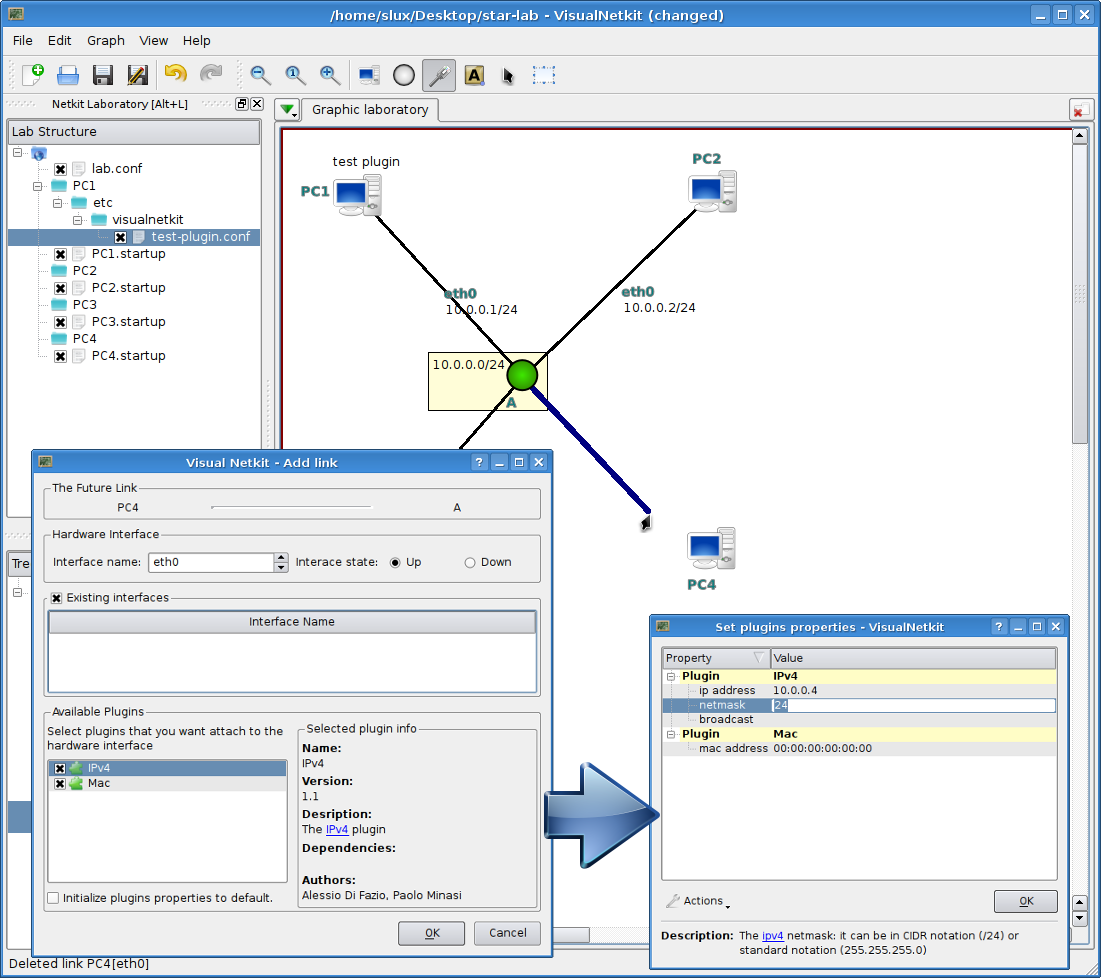
\includegraphics[width=12cm]{images/vnetkit_example3.png}
	\caption{Inserimento dei links.}
	\label{figura:vn_ex_links}
\end{figure}

Al termine dell'operazione è possibile inserire il dominio di collisione posto a ``centro stella'', che andrà a collegare tutti gli host virtuali precedentemente creati. In fine, il lavoro sarà completato dall'inserimento dei links in cui verranno attivati i \plugin{} \emph{IPv4} e \emph{MAC}. Figura \ref{figura:vn_ex_links}.

Una volta realizzata la topologia di rete desiderata, il tool permette l'aggiunta di aree che possono essere utilizzate come etichette, oppure come aggregatori di elementi.

\section{Caso di studio 2: configurazione avanzata di una rete}
Terminata la fase di creazione della topologia di rete desiderata, l'utente spesso ha la necessità di configurare i servizi presenti all'interno degli host virtuali. \visualnetkit{} offre questa possibilità mediante l'uso della dock delle proprietà.
Quando si seleziona un elemento della scena grafica - doppio click -, il sistema provvede a renderizzare le informazioni dell'oggetto all'interno della property dock. Possiamo quindi trovare tutte le propietà presenti all'interno dei \plugin{} attivi per l'entità selezionata.

Alcuni moduli più complessi (nel caso dell'esempio il \plugin{} \emph{Test}) prevedono la possibilità di poter manipolare la struttura delle properties, in particolare inserendo o eliminando sotto-attributi (figura \ref{figura:vn_ex_pp}).

\begin{figure}[!htb]
	\centering
	\includegraphics[width=13cm]{images/vnetkit_property_evolution.png}
	\caption{Modifica della struttura delle properties di un \plugin{}.}
	\label{figura:vn_ex_pp}
\end{figure}
Si vuole quindi modificare la struttura del modulo \emph{Test} attivo sulla macchina virtuale ``PC1''. Come mostrato, viene prima inserata una sotto-proprietà dell'attributo ``property-1'', successivamente si tenta di inserire tre copie della proprietà ``property-2'' che il modulo prevede.
Al tentativo di inserimento della quarta copia di quest'ultima, il \plugin{} restituisce un errore in quanto non sono previste più di tre duplicati per la proprietà in esame.

Quindi, tramite l'apposito bottone ``Actions'' è possibile, per ogni proprietà di un modulo eliminare o aggiungere le sotto-property quando consentito. Quest'ultimo controllo - come quello inerente al controllo di cardinalità di una property poc'anzi citato - è interamente affidato al \plugin{}.

Il modulo utilizzato nell'esempio è puramente utilizzato per il testing. Tuttavia si può facilmente immaginare che un \plugin{} che offra un servizio complesso (come Zebra o Quagga) possa avere una struttura simile a quella mostrata, ossia che contenga molteplici attributi con una struttura gerarchica complessa.

\section{Caso di studio 3: sperimentazioni sul laboratorio creato}
Lo stadio finale della costruzione di un laboratorio mediante l'utilizzo di \visualnetkit{} si conclude con il salvataggio dello stesso sul \fs{}. Mediante la voce \emph{Save As\ldots} presente nel menu \emph{File} è possibile selezionare la directory dove il Lab creato verrà memorizzato.

Effettata questa operazione si può provvedere anche alla chiusura di \visualnetkit{}. Da questo momento in poi viene utilizzato \netkit{}\footnote{La spiegazione di come avviare un laboratorio con \netkit{} va oltre gli obiettivi di questo lavoro.} per avviare la rete virtuale, dove è possibile effettuare tutti i test che si desiderano.


	
	%%%%%%%%%%%%%%%%%%%%%%%%%%%%%%%%%%%%%%%%%
	% CAPITOLO 5
	%%%%%%%%%%%%%%%%%%%%%%%%%%%%%%%%%%%%%%%%%
%	\include{capitoli/cap5}
	
	%%%%%%%%%%%%%%%%%%%%%%%%%%%%%%%%%%%%%%%%%
	% CONCLUSIONI
	%%%%%%%%%%%%%%%%%%%%%%%%%%%%%%%%%%%%%%%%%
	% Elimino l'intestazione della pagina per le conclusioni e la bibliografia
	\rhead{}
	\lhead{}	
	\renewcommand{\headrulewidth}{0pt}
	
	\chapter*{Conclusioni}
% Inserisce la voce di questo capitolo nell'indice
\addcontentsline{toc}{chapter}{Conclusioni}

TODO
	
	%%%%%%%%%%%%%%%%%%%%%%%%%%%%%%%%%%%%%%%%%
	% RINGRAZIAMENTI
	%%%%%%%%%%%%%%%%%%%%%%%%%%%%%%%%%%%%%%%%%
	\chapter*{Ringraziamenti}
% Inserisce la voce di questo capitolo nell'indice
\addcontentsline{toc}{chapter}{Ringraziamenti}

A Michela per il suo impagabile sostegno e aiuto.\\
\\
A tutti gli amici con i quali ho condiviso questi anni universitari.\\
\\
A Dario per avermi fatto avvicinare al mondo open-source.\\
\\
Al Prof. Maurizio Pizzonia e Massimo Rimondini che mi hanno dato la possibilità di svolgere questo lavoro.\\
\\
Ed infine, a tutti i professori del Dipartimento di Informatica e Automazione (\emph{D.I.A.}) dell'Università degli studi di ``Roma Tre'', che con estrema professionalità hanno sempre svolto il proprio lavoro egregiamente.

	
	%%%%%%%%%%%%%%%%%%%%%%%%%%%%%%%%%%%%%%%%%
	% BIBLIOGRAFIA
	%%%%%%%%%%%%%%%%%%%%%%%%%%%%%%%%%%%%%%%%%
	\clearpage
% Inserisce la voce di questo capitolo nell'indice
\addcontentsline{toc}{chapter}{Bibliografia}
\begin{thebibliography}{9}
\bibitem{OSSINI}
	M. Zec, M. Mikuc.
	\emph{Operating System Support for Integrated Network Emulation in IMUNES}, to appear in Proceedings of the 1st Workshop on Operating System and Architectural Support for the on demand IT InfraStructure / ASPLOS-XI, Boston, October 2004.

\bibitem{MVNL08}
	Jean-Vincent Loddo, Luca Saiu.
	\emph{Marionnet: A Virtual Network Laboratory and Simulation Tool}, SimulationWorks, Marseille (France), 2008

\bibitem{QUATC05}
	Fabrice Bellard.
	\emph{QEMU, a Fast and Portable Dynamic Translator}, 2005 USENIX Annual Technical Conference.

\bibitem{VNUMLT}
	\emph{VNUML Tutorial}, www.dit.upm.es/vnumlwiki/index.php/Tutorial.

\bibitem{VNUMLGUI}
	\emph{VNUMLGUI}, pagesperso.erasme.org/michel/vnumlgui.

\bibitem{NETKIT}
	\emph{Netkit}, www.netkit.org.

\bibitem{IRPI07}
	Massimo Rimondini.
	\emph{Interdomain Routing Policies in the Internet: Inference and Analysis}, A thesis presented by Massimo Rimondini in partial fulfillment of the requirements for the degree of Doctor of Philosophy in Computer Science and Engineering, Roma Tre University, Dept. of Informatics and Automation, March 2007.

\bibitem{ECNN07}
	Massimo Rimondini.
	\emph{Emulation of Computer Networks with Netkit}, Tutorial held during the 4th International Workshop on Internet Performance, Simulation, Monitoring and Measurement (IPS MoMe 2006) in Salzburg, February 2006.

\bibitem{AUPL04}
	Craig Larman.
	\emph{Applying UML and Patterns: An Introduction to Object-Oriented Analysis and Design and Iterative Development (3rd Edition)}, Prentice Hall PTR, October 2004.

\bibitem{SSA06}
	Nick Rozanski, Eoin Woods
	\emph{Software System Architecture: Working With Stakeholders Using Viewpoints and Prespectives}, Addison Wesley

\end{thebibliography}

	
\end{document}

%%%%%%%%%%%%%%%%%%%%%%%%%%%%%%%%% DOCUMENTO - FINE %%%%%%%%%%%%%%%%%%%%%%%%%%%%%%%%%%%%%%%%%%%%%%%%%%
